\chapter{Tonal placement in adverse phonological environments}
\section{Introduction}
Tonal placement in words containing vowels and sonorant consonants is to some extent systematic, but, at the same time, characterised by a high degree of variability. On the one hand, the data suggest a systematic alignment of the pitch peak with a certain structural unit (here the syllable nucleus). On the other hand, the choice of which syllable nucleus the pitch peak co-occurs with is prone to a vast amount of variability. Beyond words containing vowels and sonorant consonants, Tashlhiyt offers the rare possibility to look at tonal placement in absence of voiced material. Although there is much cross-linguistic work on tonal placement in contexts that are impoverished in terms of voiced material (cf. Chapter 2), these contexts usually contain at least a short vowel to carry parts of the tonal movement. The present chapter will explore tonal placement in words where sonorant material is completely absent, i.e. in words that are comprised of obstruents only.\is{tonal alignment} 

The chapter is structured as follows. First, we will present a qualitative exploration of tonal placement in words containing obstruents only based on Grice et al.’s findings (\citeyear*{Grice.etal2015tash}) (\sectref{sec:6.2}). We will show that there are three different patterns: the pitch peak either remains unrealised (no noticeable pitch movement), occurs on the vowel of the preceding word, or, crucially, occurs on a non-lexical central vowel. This central vowel will be henceforth referred to as schwa. In the last two decades, schwa in Tashlhiyt has been subject to extensive debates with regard to its linguistic status (or the lack thereof). After reviewing the literature surrounding the debate on schwa (\sectref{sec:6.3}), we will present evidence that sheds new light on schwa and its role within Tashlhiyt’s linguistic system (\sectref{sec:6.4}). Finally, we will discuss the results in light of the available literature and conclude with a revised evaluation of the status of schwa in Tashlhiyt (\sectref{sec:6.5}).

\section{Tonal placement in absence of sonorants}\label{sec:6.2}
\citet{Grice.etal2015tash} report on tonal placement on target words containing neither a lexical vowel nor a sonorant consonant (e.g. /tb̩.dg̍/ ‘she was wet’). These words exhibited an exceptional degree of variability resulting in tonal placement patterns that diverged considerably from words with sonorants. Three patterns were observed: first, in some utterances the pitch peak remained unrealised (no noticeable pitch movement). This is henceforth referred to as ‘no surfacing tone'. Second, the pitch peak was produced on the vowel in the previous word, i.e. on /a/ of /inna/. This pattern is henceforth referred to as ‘anticipated tone'. Thirdly, the pitch peak was sometimes realised on a schwa-like non-lexical vowel in word-medial or word-final position. This pattern is henceforth referred to as ‘tone on schwa'. Which pattern was used was to some extent speaker dependent. However, all speakers showed instances of all three patterns and all three patterns were found for both questions and contrastive statements. The schematic representation of these strategies is displayed in \figref{fig:6.1} and production examples are illustrated in \figref{fig:6.2} and \figref{fig:6.3}.

  \begin{figure}
   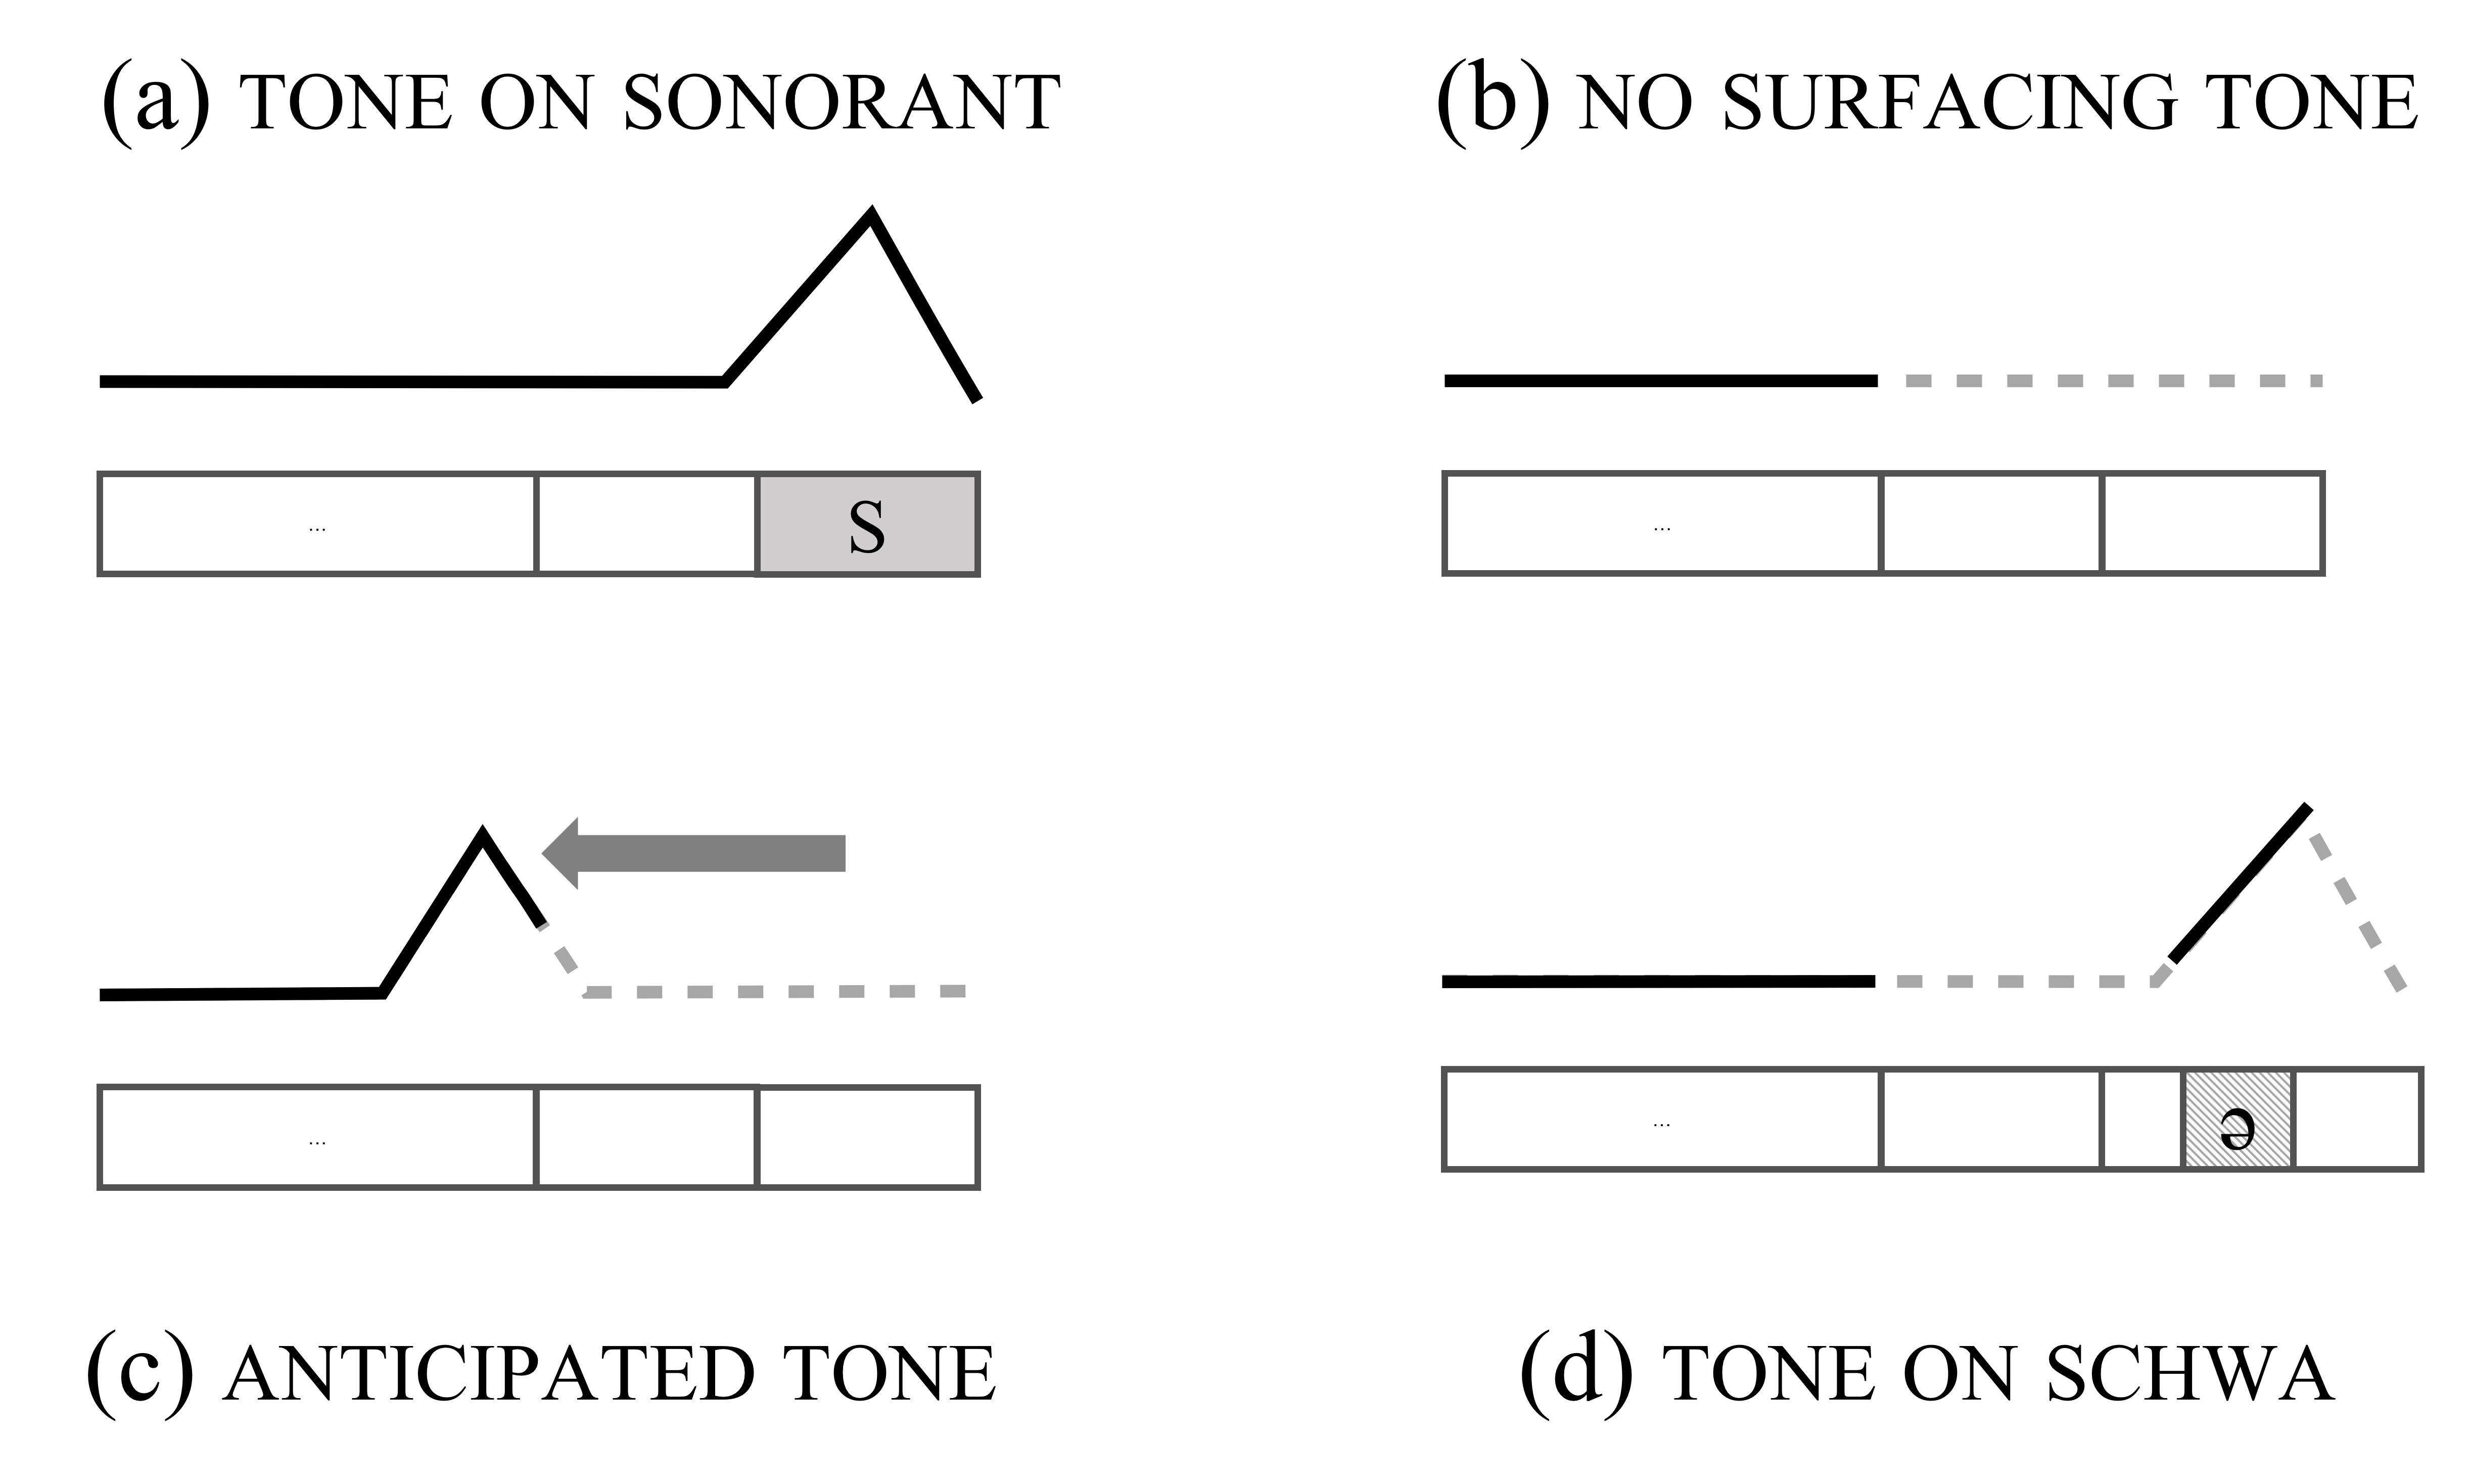
\includegraphics[width=1\textwidth]{figures/Figure_6_1.png}
  \caption{Schematic representation of tonal placement patterns observed in phrase-final words with a sonorant nucleus (a) and with obstruent nuclei only (b-d). In (b) the pitch peak is not realised; in (c) the pitch peak is realised on the final vowel of the preceding word; and in (d) the pitch peak surfaces on a schwa. }
   \label{fig:6.1}
   \end{figure}

  \begin{figure}
   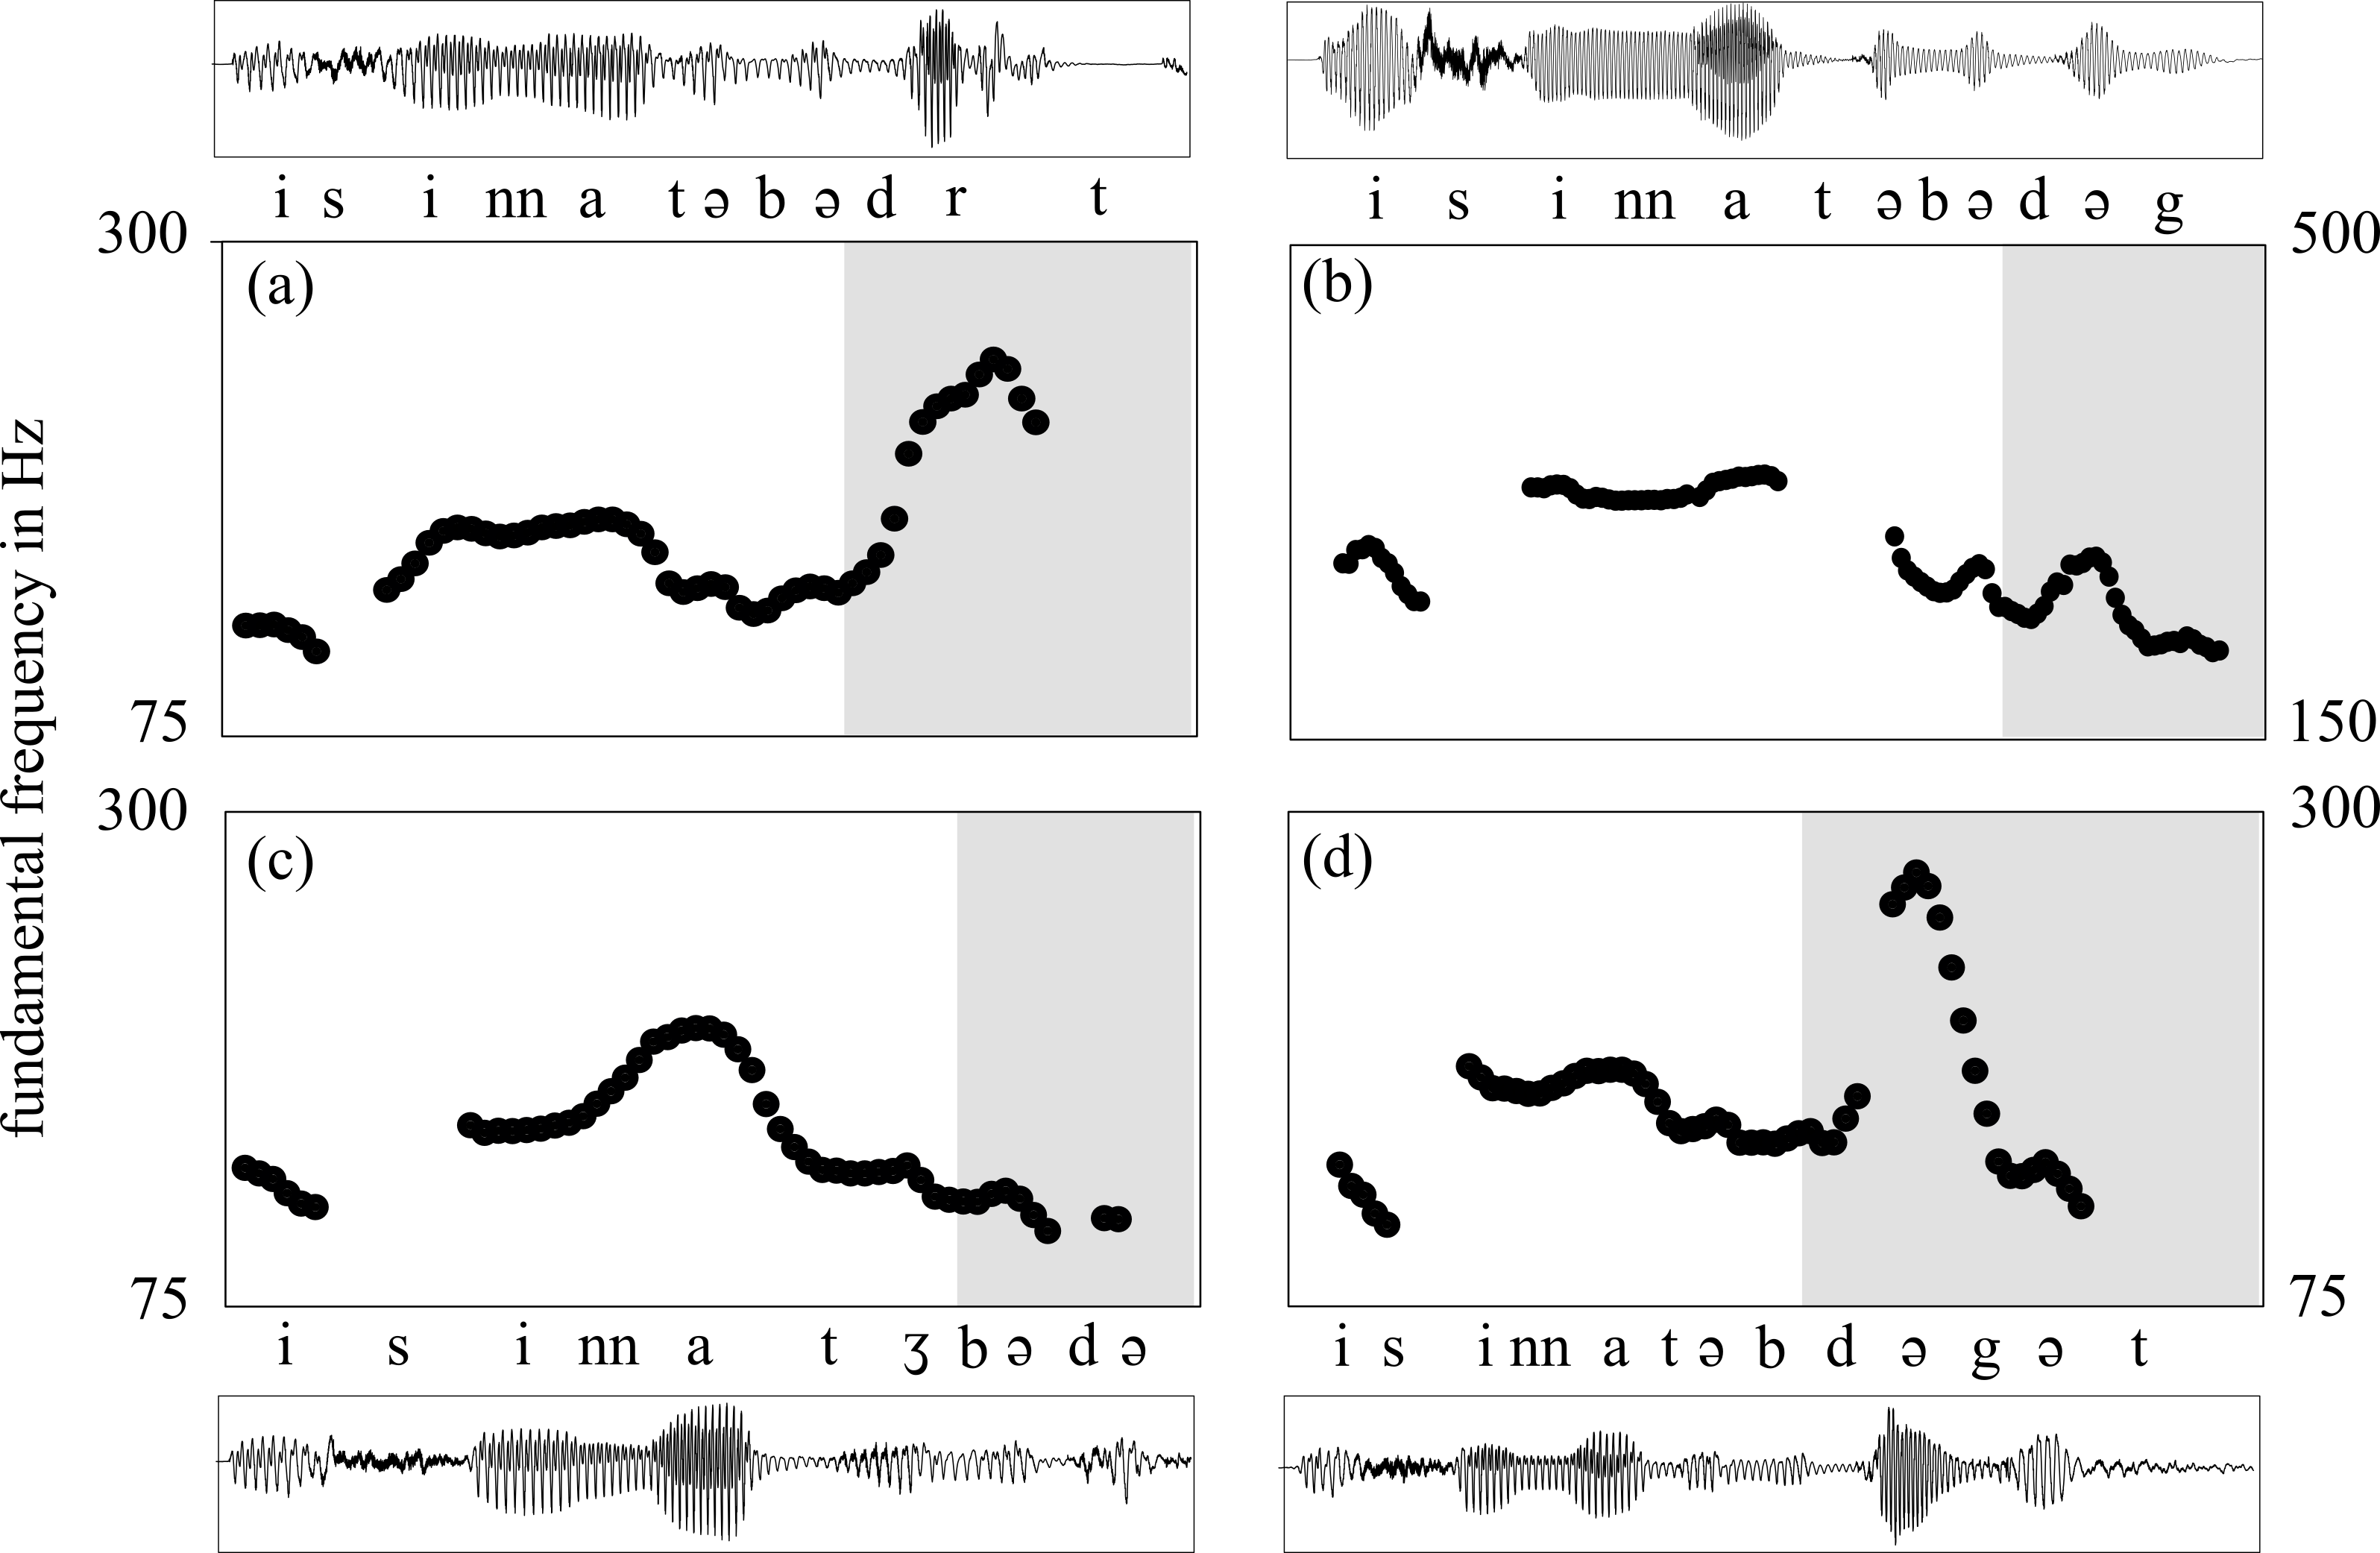
\includegraphics[width=1\textwidth]{figures/Figure_6_2.png}
  \caption{Representative waveforms and f0 contours of y/n questions /is inna (a) tbdr, (b) tbdg, (c) tjbd, (d) tbdgt/ ‘Did he say ‘she mentioned’, ‘she was wet’, ‘she pulled’, ‘you were wet’? (a) illustrates an utterance with a sonorant nucleus (/r/); (b) illustrates a production without any residual of the pitch peak; (c) illustrates a production of the pitch peak being anticipated and realised on the preceding word; (d) illustrates a production of the pitch peak being realised on a schwa. Final syllables are highlighted in grey.}
   \label{fig:6.2}
   \end{figure}

  \begin{figure}
   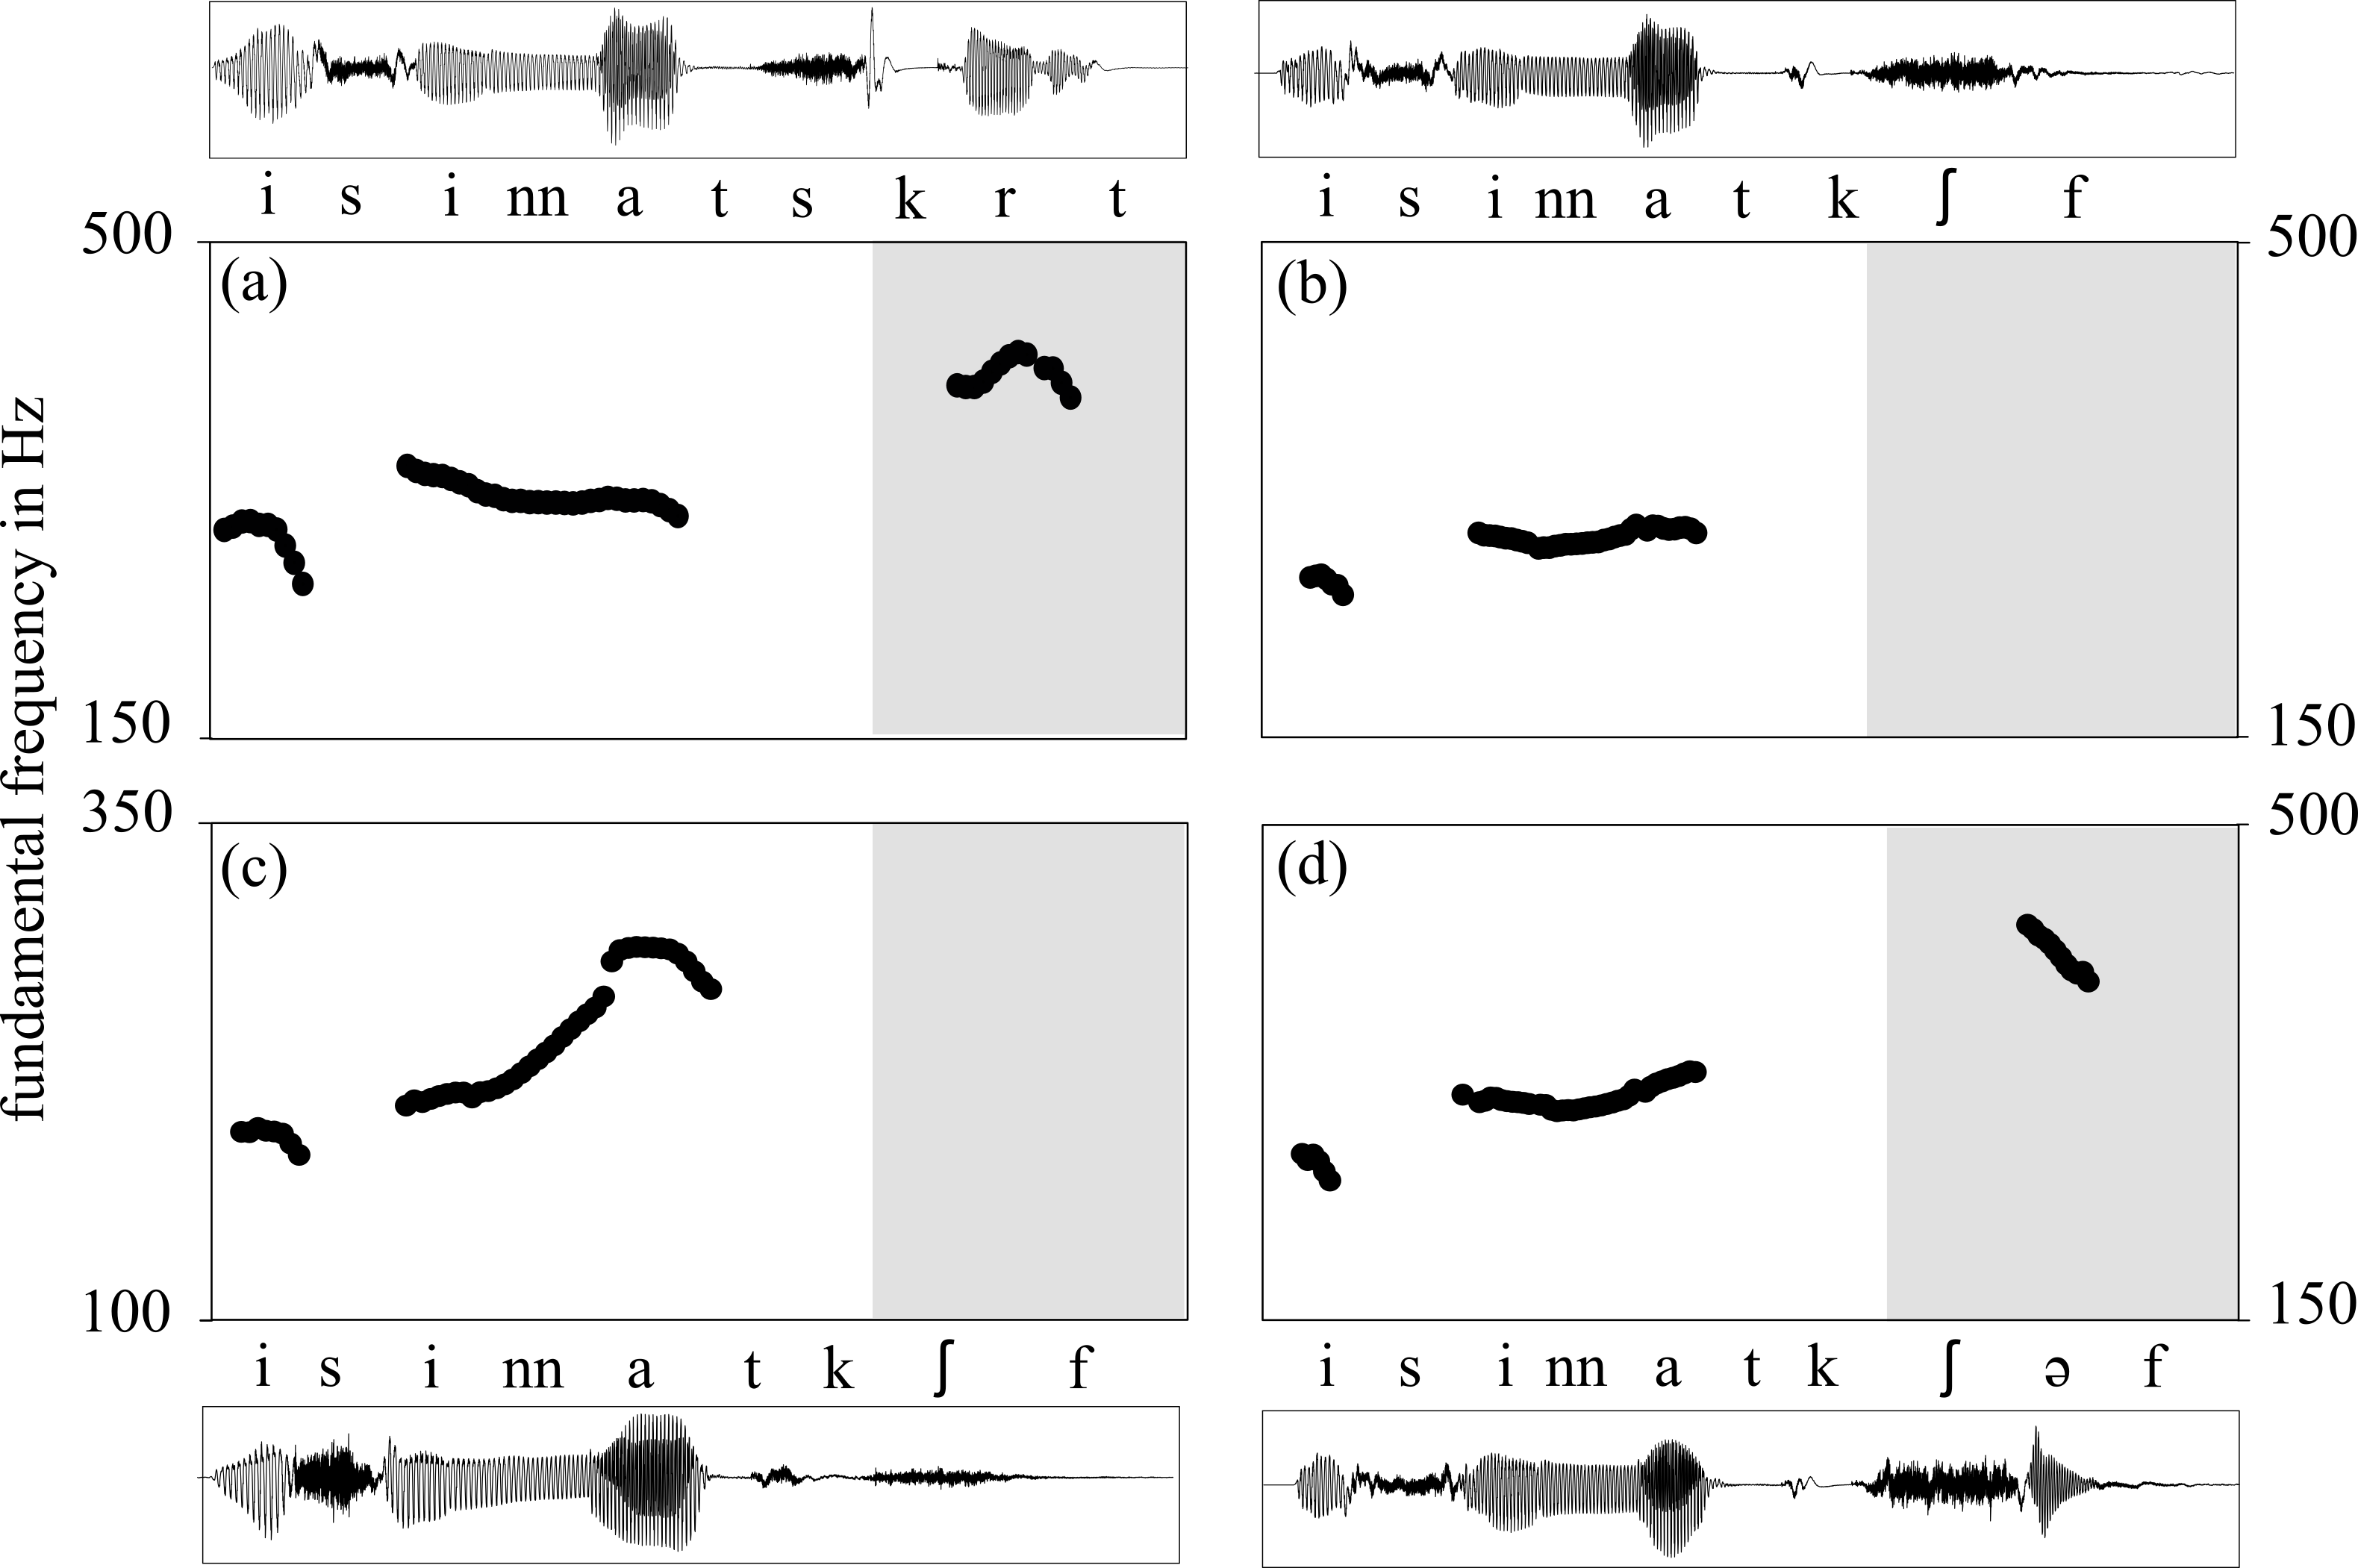
\includegraphics[width=1\textwidth]{figures/Figure_6_3.png}
  \caption{Representative waveforms and f0 contours of y/n questions: /is inna (a) tkʃf, (b-d) tskrt?/ ‘Did he say ‘it dried’, ‘you did’? (a) illustrates an utterance with a sonorant nucleus in a voiceless environment (/r/); (b) illustrates a production without any residual of the pitch peak; (c) illustrates a production of the pitch peak being anticipated and realised on the preceding word; (d) illustrates a production of the pitch peak being (partly) realised on a schwa. Final syllables are highlighted in grey.}
   \label{fig:6.3}
   \end{figure}

As can be seen in \figref{fig:6.2}b, when the phrase-final word does not contain a sonorant, the pitch peak can remain unrealised exhibiting no noticeable pitch peak (no surfacing tone). Importantly, the target word (/tb̩.dg̍/ ‘she was wet’) contains voiced segments and it even surfaces frequently with schwa-like elements between consonants. Thus, phonetically, the word is able to carry a tonal movement.\footnote{Note that the small bumps in f0 on /tbdg/ are caused by microprosodic perturbations. They do not give rise to the perception of a tonal movement (cf. respective sound files).}

In the anticipated tone pattern, the tone was shifted to the left resulting in the pitch peak occurring on the final vowel of /inna/. Similar to the no surfacing tone pattern, the target word (/tj̍.bd̩/ ‘she pulled’) exhibits clear voicing, but does not bear the pitch peak (\figref{fig:6.2}c). The no surfacing tone pattern and the anticipated tone pattern were only found in utterances containing target words comprised of obstruents only. It is never observed in utterances with target words containing sonorants.\is{tonal shift} 

In the tone on schwa pattern, the pitch peak was realised on a schwa-like non-lexical vowel (\figref{fig:6.2}d). Although it is not the final vocoid in the word, schwa between /d/ and /g/ carries significant parts of the rise-fall in pitch. The same patterns of tonal placement are found for phrase-final words containing voiceless obstruents only, as illustrated in \figref{fig:6.3}. 

Most importantly, in words containing only voiceless obstruents, the anticipated tone and the presence of a schwa were mutually exclusive, i.e. when the pitch peak was anticipated, no schwa occurred in the target word; and vice versa, if there was a schwa in the target word, it carried the pitch peak. Thus, tonal placement in voiceless environments exhibits a discrete alternation dependent on the availability of a schwa. This suggests a structural function of this schwa. However, as certain authors have argued, the phonological status of schwa in Tashlhiyt is questionable. The placement of tones on schwa and, in turn, its linguistic status appears to be a key in understanding tonal placement in its entirety. Thus, the following section will summarise the literature on this topic.

\section{The status of schwa in Tashlhiyt: a review}\label{sec:6.3}
Schwa and its role in the phonological system of Tashlhiyt has sparked a heated debate lasting for over two decades. \citet{Coleman1996,Coleman1999,Coleman2001} considers schwa as a phonological element epenthesised by the phonological component to repair illicit syllable structure. This account will be referred to as the ‘epenthetic vowel account'. Contrary to this approach, several authors have claimed that schwa has no phonological relevance for the linguistic system whatsoever (\citealt{DE1985,DE1996,DE2002,DE2008,Ridouane2008,FougeronRidouane2008,RidouaneFougeron2011}). These authors treat these vocalic elements as transitional vocoids – phonetic artifacts caused by the dynamics of speech articulation. The occurrence of schwa is assumed to be largely predictable from the laryngeal and supralaryngeal specification of its consonantal environment. This account will be referred to as the ‘transitional vocoid account'. The two mentioned views correspond roughly to the typology of inserted vowels proposed by \citet{Hall2006} which assumes a clear-cut division between inserted vowels that are phonological units and those that are not. This assumption is based on traditional linguistic models that consider ‘phonetics' and ‘phonology' as separable subsystems. More recent models incorporate distributions of variation that do not require such a categorical distinction between phonetics and phonology. For the sake of discussing the relevant literature, we will stick to the categorical view put forward by the involved authors. The epenthetic vowel account and the transitional vocoid account differ mainly in their predictions with regard to schwa’s interaction with phonological patterns and its distribution within the word. In the following, both accounts will be discussed and compared.\is{vowel insertion} 

\subsection{The epenthetic vowel account}
Coleman (1996, 1999, 2001) treats interconsonantal schwas as epenthetic segments, interpreting syllabic consonants in Dell and Elmedlaoui’s model (e.g., /b̩/ and /g̍/ in /tb.̩dg̍̍/ ‘she was wet’) as sequences of a phonological schwa plus consonant (/təb.dəg/). In his model, epenthetic schwas are expected to occur in any syllable nucleus position that is not occupied by one of the lexical vowels /a, i, u/. Schwa is argued either to acoustically surface as a central vowel (as in the case of [təbdəg]), or not to surface due to articulatory overlap of adjacent consonantal gestures. According to Coleman, the assumed underlying schwa in the first syllable in /təs.ti/ ‘she selected’ does not surface because it is completely overlapping with the surrounding consonants resulting in [tsti]. This leaves differing acoustic realisations to variability in the phonetic implementation of the epenthetic vowel. \is{vowel insertion}\is{gestural coordination} 

The most important arguments in favour of this analysis come from the acoustic study presented in \citet{Coleman2001}. He analysed recordings of one Tashlhiyt speaker producing 654 target words in a carrier phrase (/ini za \textsc{target} tklit adˀnˀi(nˀ)/ ‘please say \textsc{target} again’). He counted the occurrences of schwa and measured duration and the first three formants (among other parameters). First, Coleman compared how well his account predicted the presence of schwa in comparison to a phonetic account (concretely referring to \citealt{DE1996}). Comparing the goodness-of-fit between the observed distribution of schwa and their expected occurrence according to the two models, Coleman reports on slightly better fits of his model compared to Dell and Elmedlaoui’s model. Coleman further discusses cases of schwa that are problematic for Dell and Elmedlaoui’s account. For instance, he reports on productions of a schwa in word-final position (e.g. [tbdgə]). This word-final schwa can obviously not be considered as a mere transition between consonantal gestures but, according to Coleman, can be considered as a realisation of a syllable nucleus in word-final position. In addition to distributional arguments, he claims that the quality of schwa is, while highly dependent on its consonantal context, not entirely predictable by adjacent consonants.\is{vowel insertion}\is{gestural coordination} 

To summarise Coleman’s position in this debate, he considers neither the presence of schwa nor its acoustic properties as entirely predictable from the consonantal environment. Even though he admits that Tashlhiyt has syllabic consonants at the phonetic surface, he considers it as not necessary to treat them as phonological syllable nuclei. He concludes that schwa elements are better explained as acoustic reflexes of syllable nuclei not occupied by lexical vowels. 

\largerpage
\subsection{The transitional vocoid account}
Opposed to Coleman’s view, a number of authors have argued that schwa is not a phonological element but a mere epiphenomenon of the coordination of oral and laryngeal gestures. Support for this view can be subsumed under two types of arguments, phonological and distributional in nature. 

\subsubsection{Phonological arguments}
Tashlhiyt Berber has a strong musical tradition. One particular type of verse form is the ‘Rrways’ (cf. \citealt{schuyler1979}). One characteristic of Rrways is the uniformity of lines, in other words, all lines are sung to the same tune, resulting in lines with identical metre. A metre is defined as a specified sequence of two types of syllables: light syllables, defined as syllables lacking a coda consonant (e.g. /ma/) and heavy syllables, defined as syllables with a coda consonant (e.g. /mat/). 

\begin{exe}
\ex\label{ex:6:1} \begin{xlist}
                \ex\label{ex:6:1a} tʃ ʃit tswit \newline
                tʃ. ʃi.(t)ts.wit \newline
                ‘you have enough to eat and to drink’
                \ex\label{ex:6:1b} tlsit dʒin \newline 
				tl.si.td.ʒin \newline	
				‘you wear Jean’s trousers’
				\ex\label{ex:6:1c} tasit lquq  \newline 
				ta.si.tl.quq \newline	
				‘you have a girlfriend’
                \ex\label{ex:6:1d} ma ssul trit \newline 
				ma.(s)su.lt.rit \newline	
				‘what else do you want?’  
\end{xlist}
\end{exe} 

The four lines in \REF{ex:6:1} have the same meter characterised by a sequence of three light syllables followed by one heavy syllable (cf. \tabref{tab:6.1}, taken from \citealt{Ridouane2008}). If one compares the syllables across the first column of \tabref{tab:6.1}, it becomes apparent that syllables containing two consonants such as in line (a) and (b) (/tʃ/and /tl/) pattern with CV syllables such as in line (c) and (d) (/ta/ and /ma/). In other words, a sequence of two consonants, analysed by Dell and Elmedlaoui as an open syllable with a consonant in nucleus position, is considered metrically equivalent to a sequence of a consonant plus vowel, constituting a light syllable. On the other hand, consider the possibility that syllables containing two adjacent consonants contain a schwa, illustrated in line (a2) and (b2) (cf. \tabref{tab:6.1}).\is{syllable weight} 

\begin{table}

\caption{Metrical analysis of the verses in \REF{ex:6:1} as described in \citet[352]{Ridouane2008} and the corresponding analysis based on Coleman’s account (a2-d2) which assumes a schwa in nucleus position. Cells a2-b2 (indicated by a an asterisk) in the first columns and cells a2-d2 in the third columns illustrate mismatches of assumed phonological structures and meter in the epenthetic vowel account.}
\label{tab:6.1}
\begin{tabular}{cccccc}
\lspbottomrule
&    & \textbf{light} & \textbf{light} & \textbf{light}  & \textbf{heavy} \\
\midrule
according to       				  & \textbf{a}  & tʃ    & ʃi    & (t)ts  & wit   \\
DE (2002)	                   	  & \textbf{b}  & tl    & si    & td     & ʒin   \\
                                  & \textbf{c}  & ta    & si    & tl     & quq   \\
                                  & \textbf{d}  & ma    & su    & lt     & rit   \\
\midrule
according to 					  & \textbf{a2} & təʃ*   & ʃi    & (t)təs* & wit \\
\citet{Coleman2001}              	  & \textbf{b2} & təl*   & si    & təd*    & ʒin   \\
                                  & \textbf{c2} & ta    & si    & təl*    & quq   \\
                                  & \textbf{d2} & ma    & su    & lət*    & rit   \\
\lspbottomrule                                  
\end{tabular}
\end{table}

Syllables like /t(ə)ʃ/ and /t(ə)l/ cannot be counted as heavy syllables because they pattern metrically with CV syllables like /ta/ and /ma/ and the insertion of an actual heavy syllable at this position would lead to the ill-formedness of the tune. Instead, these syllables have to be treated as light syllables. Alternatively, in Coleman’s account, schwa has to be considered the only phonological element that does not contribute to syllable weight in the context of versification. As opposed to consonants and the bona fide vowels /i, u, a/, schwa would be an element to which the versification is blind (cf. \citealt{DE2002,Ridouane2008}). \is{syllable weight} 

Similar evidence for the lack of metrical visibility of schwa comes from the causative formation in Tashlhiyt (\citealt{Jebbour1996,Jebbour1999}). The causative is formed by prefixing either /s-/ or /ss-/ to the verb stem. According to Jebbour, the choice between the singleton and the geminate prefix depends on the moraic structure of the word. He proposes that every monomoraic verb base receives /ss-/ and every polymoraic base receives /s-/. Monomoraic bases consist of either one open syllable (e.g. /nu/ ‘to cook’ or /fl̩/ ‘to leave’) or one closed syllable with a consonantal nucleus (e.g. /rg̍l/ ‘to lock’). Polymoraic bases consist of one closed syllable with a vowel in nucleus position (e.g. /mun/ ‘to accompany’) or more than one syllable. Again, assuming a schwa in nucleus position for e.g. /fl/, i.e. assuming /fəl/ (following \citealt{Coleman2001}), schwa would not contribute to the number of moras. Note that Jebbour’s account to prosodic structure of words is somewhat incompatible with the rather simple account to versification proposed above, in which no distinction is made between syllables with a consonant and a vowel in nucleus position.\is{syllable weight} 

These metrical arguments, however, are not necessarily conclusive arguments against the epenthetic vowel account. As \citet[397]{Hall2006} acknowledges, metrical evidence is the least reliable evidence for or against the phonological status of an inserted vowel. She discusses cases in which an inserted vowel exhibits prototypical properties of a phonological vowel while, at the same time, it is invisible to the metrical system with regard to stress assignment.

In addition to metrical arguments, there are phonological alternations that provide further evidence for the non-phonological status of schwa (\citealt{Ridouane2008}). In a variety of Tashlhiyt spoken in the Anti-Atlas, the coronal stops /t, d/ surface as [s, z] when separated by one of the lexical vowels /i, a, u/ (Boukous, 1994, /tir.ʁi/  [sirʁi] ‘heat’). This alternation does not occur when the coronal stop immediately precedes another coronal consonant (e.g. /tr.ʁa/  *[srʁa] ‘it is hot’, examples from \citealt[352f.]{Ridouane2008}). If schwa is a phonological entity, it should interact with this process. According to the epenthetic schwa account (\citealt{Coleman2001}), /tr.ʁa/ should be phonologically represented as /tər.ʁa/ resulting in /t/ and /r/ not being adjacent and, in turn, enabling the assibilation process. This is not the case. Again, as opposed to the lexical vowels /i, u, a/, assibilation would be blind to schwa. 

In sum, both metrical patterns in versification, metrical patterns in causative formation, and assibilation processes do not treat schwa like lexical vowels.

\subsubsection{Distributional arguments}
The second type of argument for the non-phonological nature of schwa is based on the distribution of schwa within the word. In a direct response to Coleman, \citet{DE2002} give two important arguments counter to his account (pp. 178-187). First, there is a general disparity of observed schwa and predicted schwa in Coleman’s account. Dell and Elmedlaoui discuss the example /ts.bʁt/ ‘you painted’, which sometimes surfaces acoustically as [tsəbʁt]. The position of schwa, however, is not compatible with Coleman’s analysis in which schwas are expected between /t/ and /s/ as well as /b/ and /ʁ/, respectively (/təs.bəʁt/). Second, Coleman predicts less schwa than is actually observed. Take for example the word /tbdgt/ ‘you were wet’. According to native speakers, this word is disyllabic, thus Coleman would assume this word to be represented phonologically as /təb.dəgt/. However, in careful speech, it surfaces often as [təbədəgət]. Coleman therefore must assume two different types of schwa: one phonological schwa that occupies the syllable nucleus position and one phonetic schwa with no relevance for the phonological component. We will come back to this assumption below.

Following up on these arguments, \citet{Ridouane2008} conducted production experiments in order to instrumentally substantiate earlier claims made by Dell and Elmedlaoui. He reports on a production study, in which six native speakers read entirely voiceless words produced either in isolation (e.g. /ftχt/ ‘roll it’) or in the carrier sentence /inna jas \textsc{target} jat twalt/ ‘he told him \textsc{target} once’. Counting the number of occurrences of schwa in his corpus, he observed 18\% instances of schwa in voiceless words produced in isolation (79/432) and 4\% instances of schwa in voiceless words produced in the carrier phrase (19/432). Interestingly, the majority of observed schwas were word-final schwas (84/98, e.g. [ftχtə]) as opposed to word-medial ones (14/98, e.g. [ftəχt]). The distribution and position of these schwas were highly variable both within- and across speakers. Crucially, Ridouane argued that the distribution of these schwas is largely incompatible with Coleman’s account. In addition to the fact that there are generally few schwas to start with, he argued that those few schwas that do occur are mostly not adjacent to assumed nuclei positions in which Coleman would predict them. 

Ridouane concluded that schwa is merely an epiphenomenon of the dynamics of speech articulation exhibiting no phonological status. This conclusion was further corroborated by subsequent experiments: \citet{RidouaneFougeron2011} recorded five native speakers reading 31 words of the form C\textsubscript{1}C\textsubscript{2}VC, varying in the laryngeal specification (voiced vs. voiceless) and the manner of articulation (stop vs. fricative) of both C\textsubscript{1} and C\textsubscript{2}. Stimuli were embedded in the carrier phrase /inna \textsc{target} jat twalt/ ‘he said \textsc{target} once’. Results showed that at least two conditions should be met for what they refer to as a voiced transitional vocoid to surface acoustically: (1) the vocal tract has to be sufficiently open during the transition from one consonant configuration to the next, and (2) at least one of the consonants in the sequence should be voiced. \is{gestural coordination} 

These studies have demonstrated that the investigated transitional vocoids are highly predictable from the laryngeal and supralaryngeal specification of the consonantal environment. The authors consider schwa to be a result of gestural underlap, i.e. adjacent consonantal gestures are not entirely overlapping. Consider, for example, the cluster [dg] illustrated in \figref{fig:6.4}. \is{gestural coordination} 

  \begin{figure}
   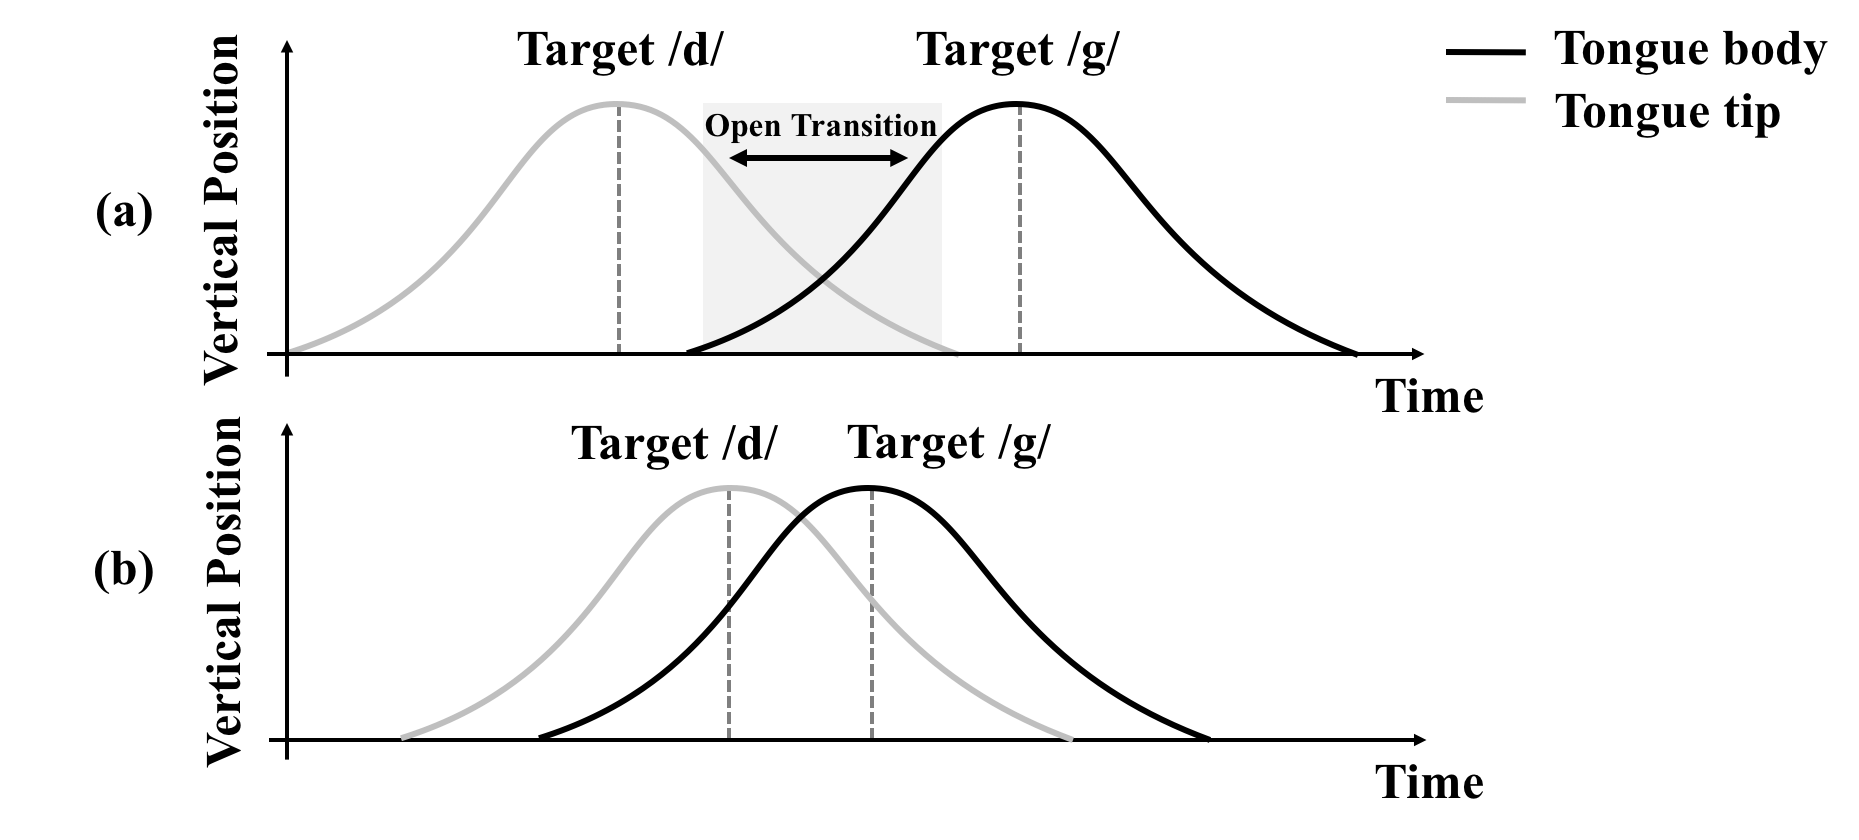
\includegraphics[width=1\textwidth]{figures/Figure_6_4_gesture.png}
  \caption{Schematic representation of the time course of articulating the cluster [dg]. In (a) there is a large lag between the constriction target of /d/ and the constriction target of /g/ resulting in an open transition. In (b), there is no open transition because the constriction targets are reached shortly after each other.}
   \label{fig:6.4}
   \end{figure}

The articulation of the [dg] cluster is characterised by two constriction gestures: the tongue tip reaches its constriction target at the alveolar ridge for [d], after which the constriction is released and the tongue body moves towards the velar region reaching a new constriction target for the [g]. The release of the first constriction has to be timed with respect to the second constriction. If the release of the first constriction takes place well before reaching the second constriction target at the velar region (cf. \figref{fig:6.4}a), there is a gestural underlap. The tongue tip has moved away from the alveolar ridge and the tongue body has not yet reached the target at the velar region. During a short period of time the vocal tract is relatively open, i.e. air can flow through the vocal tract without hindrance. The resulting open transition is accompanied by vocal fold vibration resulting in an articulatory configuration that is characteristic for vowels. The acoustic consequence is a short vowel-like articulation.\footnote{The reason for gestural underlap in Tashlhiyt might lay in the need of perceptual recoverability. In a consonant-heavy language like Tashlhiyt, consonants bear a high functional load and many acoustic cues to e.g. the place of articulation are found in the release of the consonant (\citealt{Householder1956,Malecot1958,Wang1959,Fujimura.etal1978,Ohala1990}). Overlapping constriction gestures decrease the number of acoustic cues available to distinguish the segments and, in turn, lead to diminished perceptual recoverability.}\is{gestural coordination} 

Alternatively, the consonants can overlap substantially (\figref{fig:6.4}b). The second constriction target is reached shortly after the first constriction target leaving not enough space for an open transition. Consequently, no vowel-like articulation is observed. This articulatory account is further supported by \citegen{RidouaneFougeron2011} reanalysis of articulatory data presented in \citet{FougeronRidouane2008}. In words with an acoustic schwa, they found less overlap of consonantal gestures than in words without a schwa. The discussed articulatory account is able to capture the distributional constraints discussed in \citet{RidouaneFougeron2011}. However, their account is not able to explain certain aspects of the observed data. First, it does not explain the occurrence of schwa in entirely voiceless words as reported by Ridouane (\citeyear{Ridouane2008}; see also \citealt{LoualiPuech2000}). If schwa was only an epiphenomenon of the laryngeal and oral specification of adjacent consonants, a voiced transitional vocoid is not expected to surface in voiceless environments. Second, from an articulatory point of view which only considers the timing of oral gestures, it is difficult to explain the presence of schwa in absolute final position (\citealt{LoualiPuech2000,Ridouane2008}). Third, this account does not explain the observed asymmetry between target words produced in isolation and target words produced in carrier phrases (\citealt{Ridouane2008}). \is{gestural coordination} 

In sum, even though some of the arguments for one or the other account appear to capture some facts about schwa, neither account can explain all distributional properties of those vocalic elements. The epenthetic vowel account cannot account for certain phonological regularities that are blind to the proposed epenthesised vowels. The transitional vocoid account has to face unresolved distributional anomalies that cannot be accounted for straightforwardly by a phonetic view that is based on supralaryngeal gestural coordination only. 

\section{Production study}\label{sec:6.4}
While the accounts presented above took only segmental and lower prosodic domains into account, aspects of higher prosodic domains were so far ignored. Yet, aspects of phrase-level prosodic organisation may be able to shed some more light on schwa and its role in Tashlhiyt’s phonological system. In the following, additional data from the reading task corpus introduced in Chapter 5 is analysed. The presence, distribution, and acoustic salience of schwa is explored as a function of prosodic and intonational context.

\subsection{Method}
Four sentence modalities were elicited in a reading task as discussed in detail in Chapter 5. For more details about the participants and the procedure, see section \sectref{sec:5.4}. Relevant details of the speech material, the procedure, and the analysis are repeated here. A mock dialogue was produced with the target word in phrase-final position \REF{ex:6:2} and phrase-medial position followed by an adverb \REF{ex:6:3}.

\begin{exe}
\ex\label{ex:6:2} \begin{xlist}
                \ex\label{ex:6:2a} is inna \textbf{tfsχt}?  \newline
                ‘Did he say ‘you cancelled’?’ 
                \ex\label{ex:6:2b} ur inna \textbf{tfsχt}.  \newline 
				‘He did not say ‘you cancelled’.’ 
				\ex\label{ex:6:2c} inna \textbf{ʃtf}.  \newline 
				‘He said ‘crush’.’ 
                \ex\label{ex:6:2d} manik? inna \textbf{ʃtf}? irwas. \newline 
				‘How? He said ‘crush’? It seems like it.’                
\end{xlist}
\ex\label{ex:6:3} inna \textbf{ʃtf} abadan \newline
‘He said ‘crush’ always.’
\end{exe} 

In (2a) the target word is in a y/n question. In (b) the same target word is in a negative assertion. Because of the preceding negation, a different target word is explicitly corrected in a contrastive statement in (c). Finally, in (d), the proposition in the contrastive statement is called into question in the counter-expectational echo question. Eight different target words consisting exclusively of voiceless obstruents were embedded in these sentences (see \tabref{tab:6.2}) resulting in overall 72 data points per speaker (overall 720).

\begin{table}
  \begin{tabular}{cc}
    \lsptoprule
    Target word  & Translation \\
    \midrule
ʃʃ & ‘eat'\\
ʃtf & ‘crush'\\
ftχ  & ‘roll'\\
tctft & ‘you crushed'\\
tfss & ‘she is quiet'\\
tfsxt & ‘you cancelled'\\
tkʃf & ‘it dried'\\
tsxf & ‘she fades away'\\
\lspbottomrule
  \end{tabular}
  \caption{Target words and translations of production study.}
  \label{tab:6.2}
\end{table} 

All acoustic materials were manually segmented and annotated as described in 5.4.1. The present analysis focuses on the presence of schwa. In most cases, this element was acoustically straightforward to identify (cf. \figref{fig:6.5}, \figref{fig:6.6}, and \figref{fig:6.7}, as well as corresponding sound files). In fact, it resembled acoustic realisations of lexical vowels with regard to duration and intensity. In less straightforward cases, a liberal approach of operationalising schwa was adopted. Schwa was labelled as any interval presenting periodic vibrations accompanied by a local increase in the signal energy at the consonantal release, and/or any interval after the consonantal release with formant structure or energy in the F2/F3 region characteristic of vowels.

As described in 5.4.1, productions with hesitation, unnatural phrasing patterns, and mispronunciations of the segmental material were excluded from the analyses. The amount of excluded data was substantially higher than in cases of target words containing vowels and sonorant consonants. As mentioned earlier, Tashlhiyt speakers are not used to reading aloud in their language. While care was taken to familiarise speakers with the words before the experiment, they still produced a substantial amount of mispronunciations. Only 573 of 720 utterances could be included in the statistical analysis corresponding to a data loss of 20.4\%.\footnote{Despite methodological efforts, the relatively large number of exclusions is probably still an artefact of speakers being unpractised readers of Tashlhiyt. The remaining productions, however, were judged to be natural-sounding utterances expressing the intended communicative function by independent Tashlhiyt speakers who did not participate in the experiments.}

Data was statistically analysed using R (\citealt{R}). Besides descriptive exploration of the data, the following aspects of the data set determined the choice of statistical method used here. First, the data was not intended to investigate schwa. Schwa was not expected in voiceless environments and the large number of words containing schwa came as a surprise. Second, the design was not entirely balanced (and became even less balanced due to the large amount of asymmetric data loss). Taking these factors together, it is refrained from applying statistical methods concerned with hypothesis testing. Instead, a data exploration account is taken to shed light on patterns underlying the data. 

To that end, random forests analyses are applied (\citealt{Breiman2001}), implemented by the party package (\citealt{Hothorn.etal2006,Strobl.etal2007,Strobl.etal2008}) in R (\citealt{R}). For a discussion of these techniques in the context of linguistics, see \citet{TaglBaayen2012}. Random forests analysis is a data mining technique used for classification. It is a so-called “ensemble method”. A multitude of decision trees is constructed (500 in this case). Each tree takes a set of variables and determines which variable best splits the data according to a particular criterion. Each tree is built on a random subset of variables and data. The final classification is based on the overall ensemble of trees. 

\subsection{Results and discussion}
\subsubsection{General observations}
Overall, there was an unexpectedly large amount of schwas, with 57\% of all voiceless words containing schwa. In words with schwa, there was almost exclusively only a single schwa. Schwa further occurs in all sentence modalities. \figref{fig:6.5} illustrates schwas in phrase-final words for y/n questions, negative assertions, and contrastive statements. \figref{fig:6.6} illustrates schwas in phrase-medial words for contrastive statements and corresponding echo questions. 

  \begin{figure}
   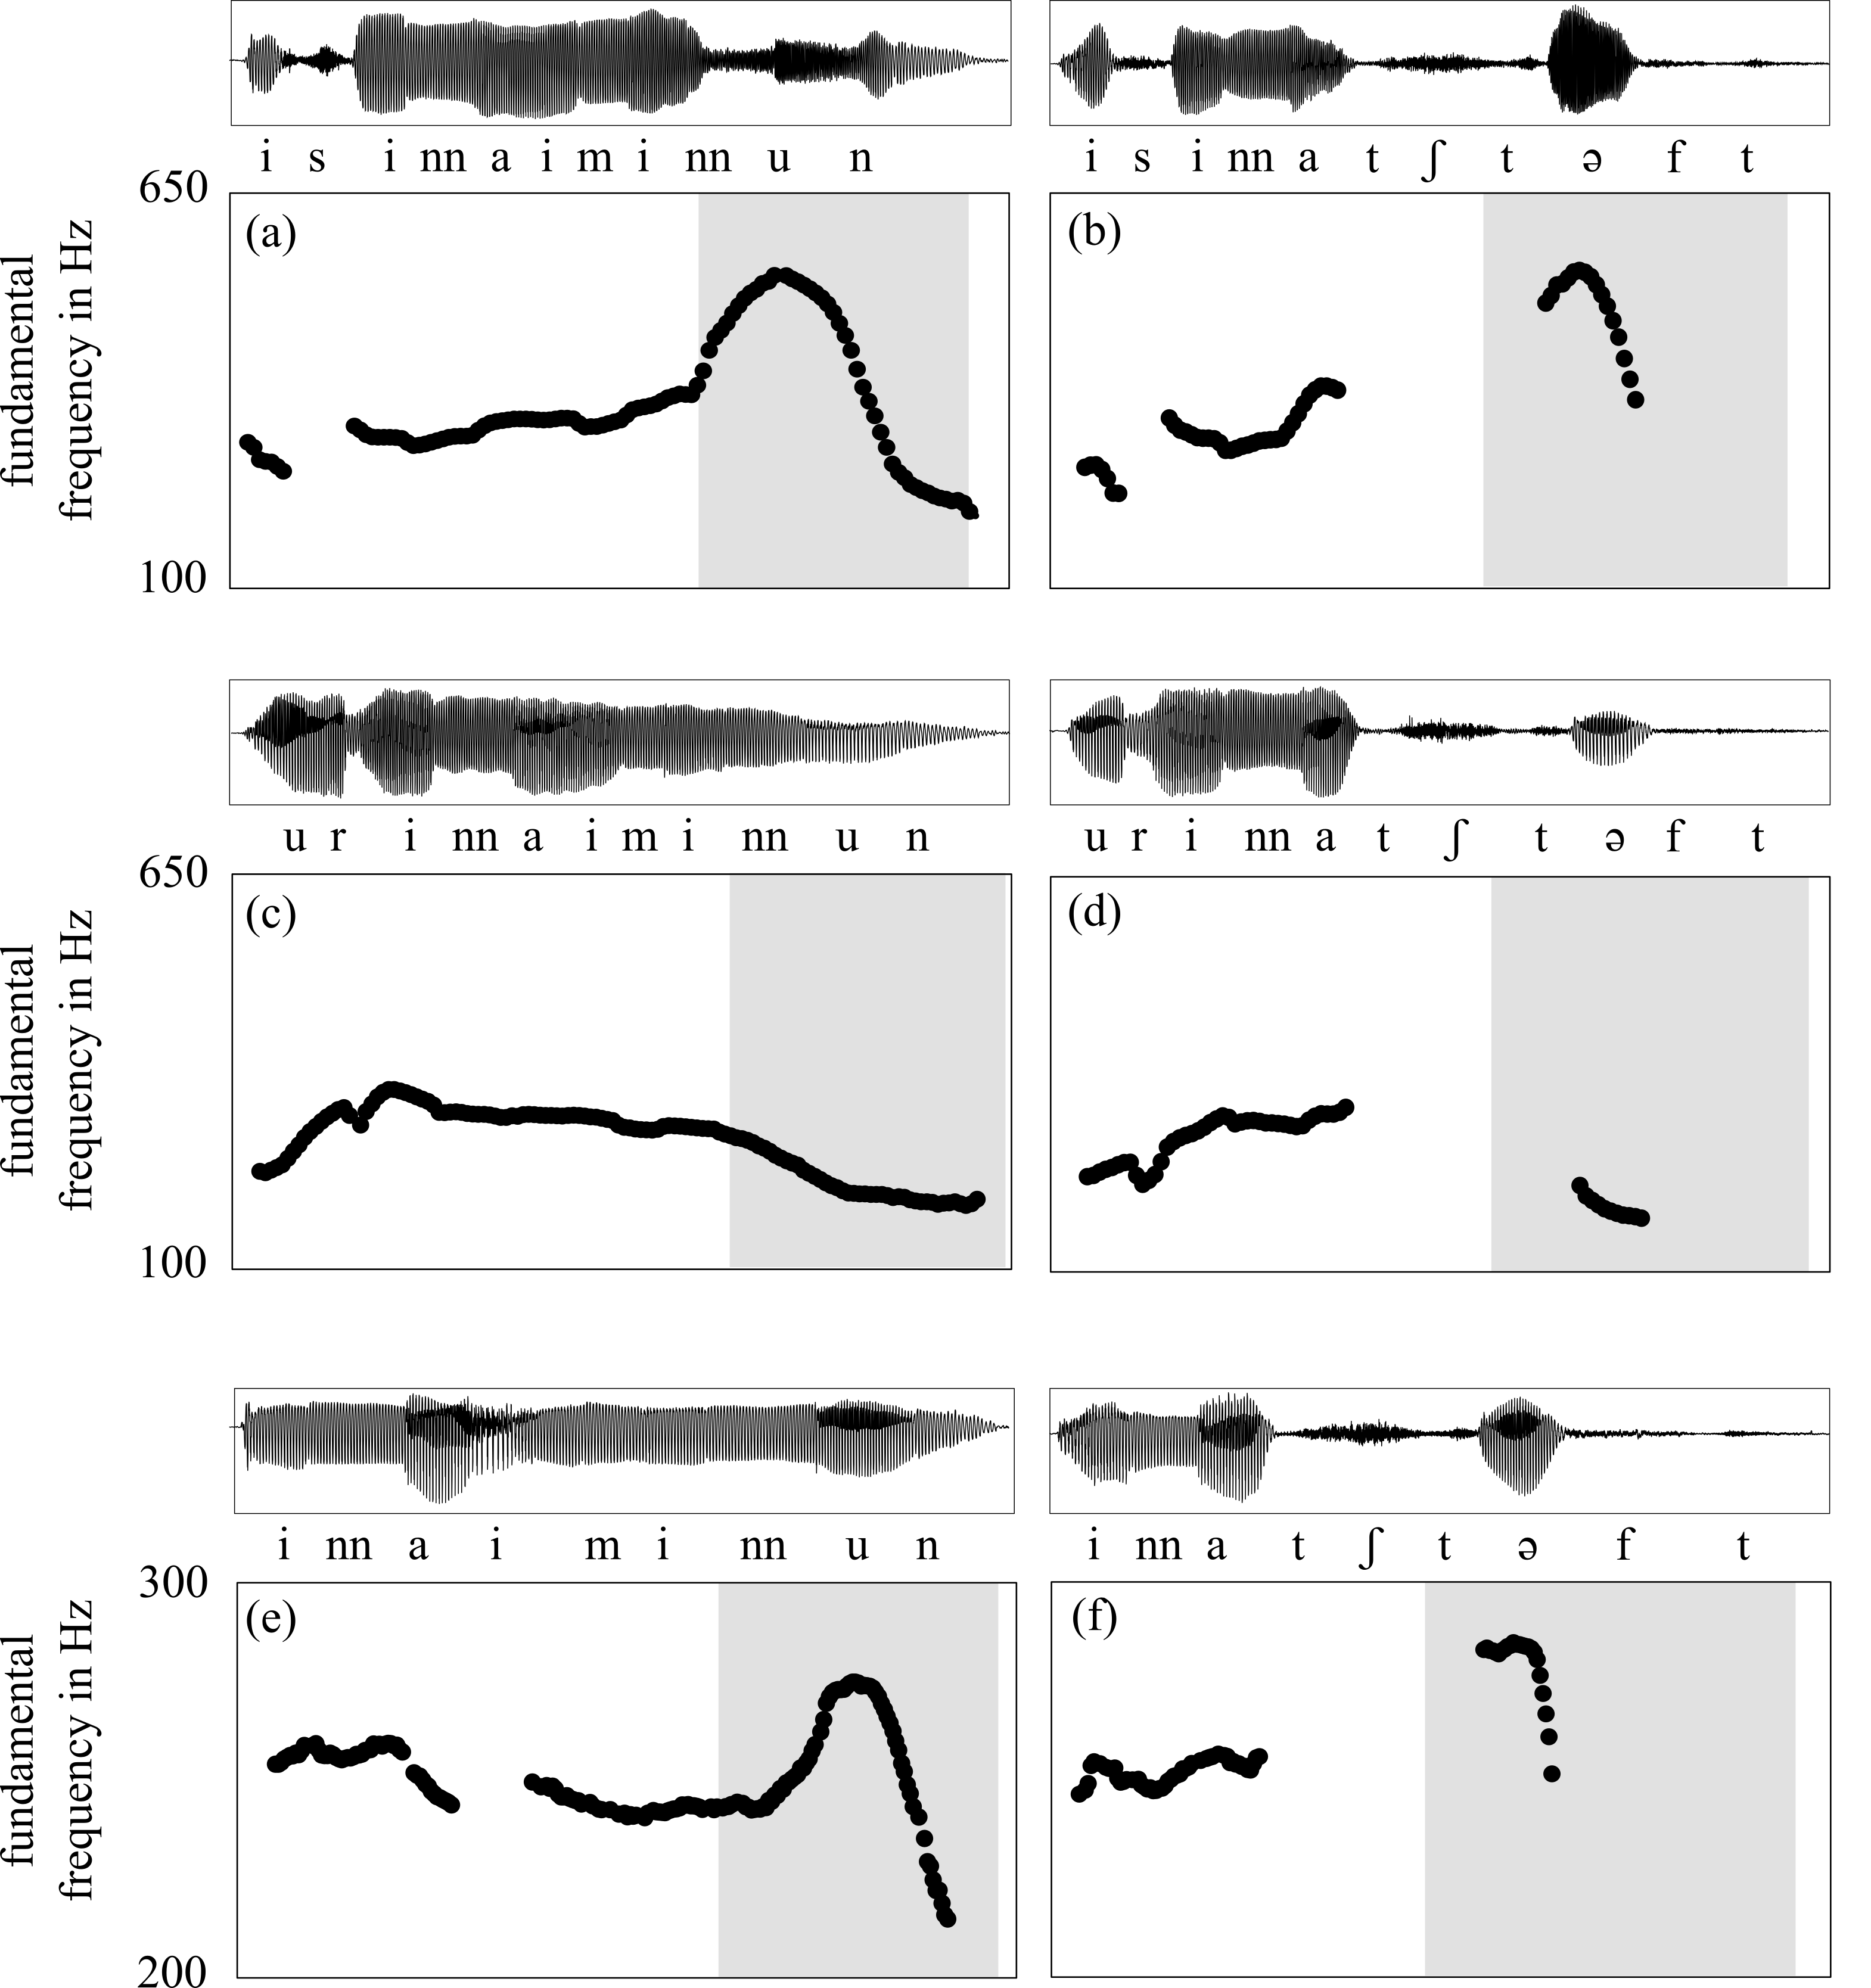
\includegraphics[width=1\textwidth]{figures/Figure_6_5.png}
  \caption{Representative waveforms and f0 contours of fully voiced utterances (target word /iminnun/, left panels) and utterances containing phonologically voiceless target words in phrase-final position (target word /tʃtft/, right panels). Top panels (a-b) display y/n questions, middle panels (c-d) display negative assertions, and bottom panels (e-f) display contrastive statements. Final syllables are highlighted in grey.}
   \label{fig:6.5}
   \end{figure}

  \begin{figure}
   
   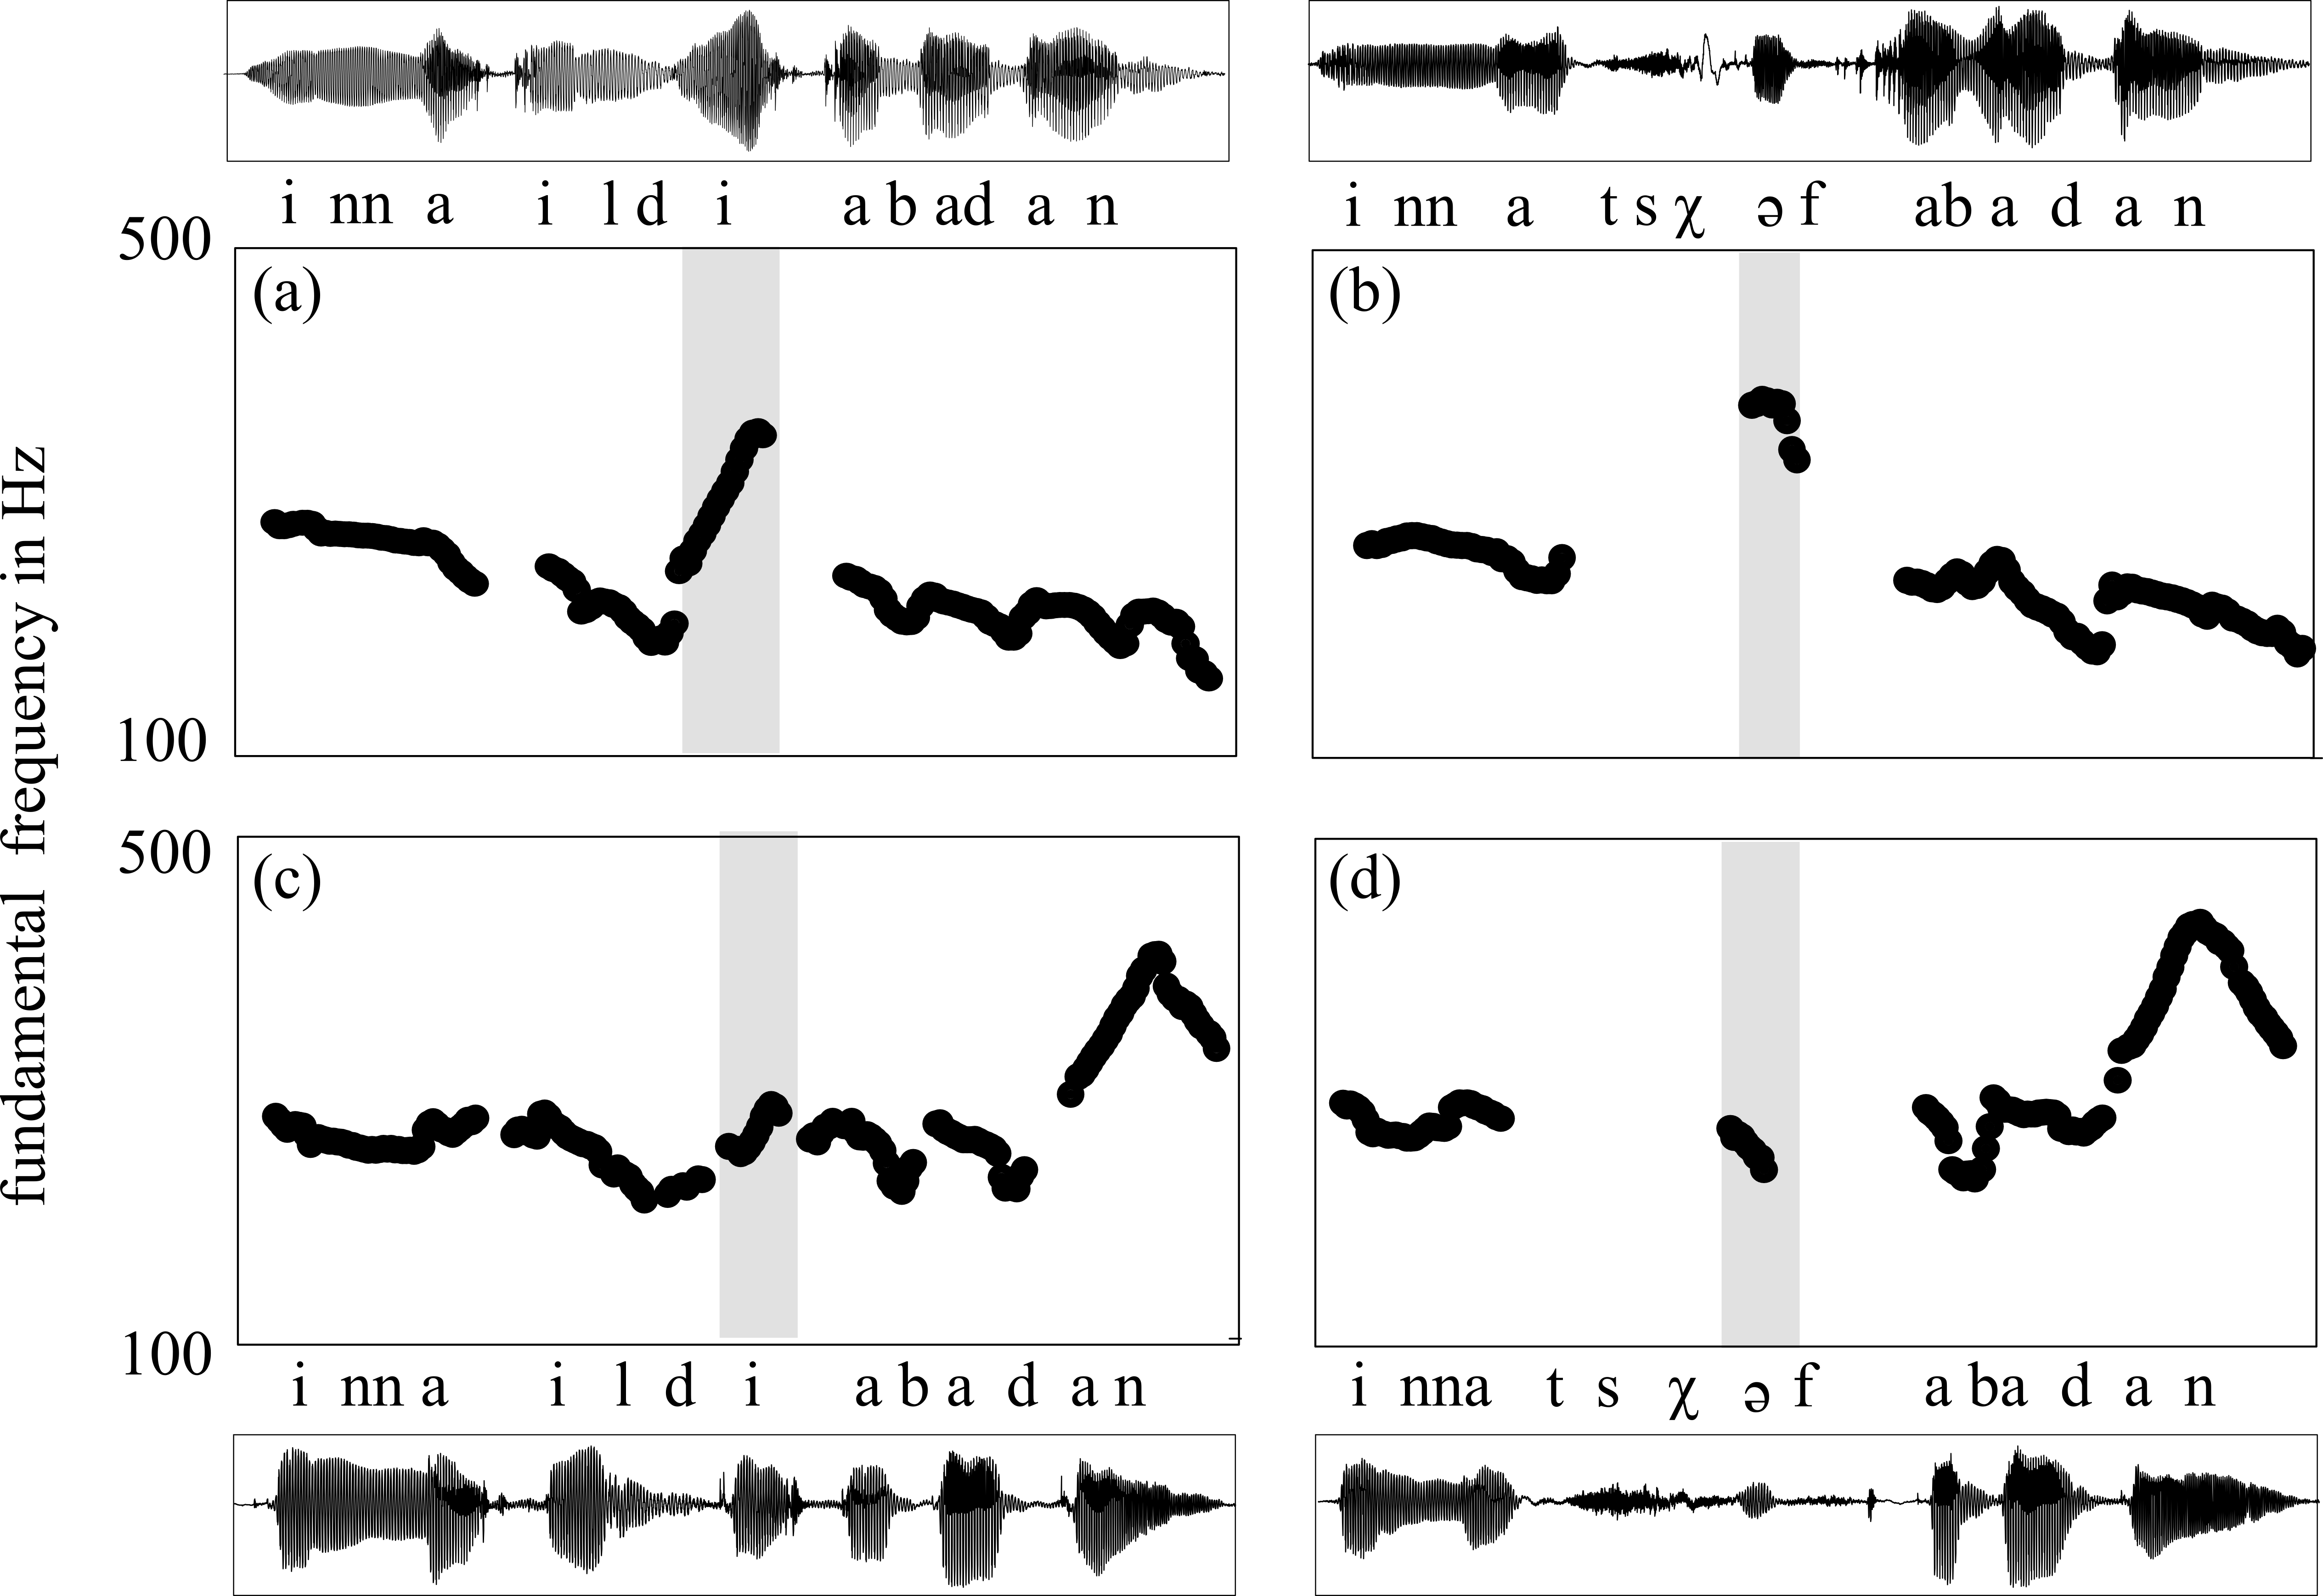
\includegraphics[width=1\textwidth]{figures/Figure_6_6_ildi.png}
  \caption{Representative waveforms and f0 contours of fully voiced utterances (target word /ildi/, left panels) and utterances containing phonologically voiceless target words in phrase-medial position (target word /tsχf/, right panels). Top panels (a-b) display contrastive statements and bottom panels (c-d) display echo questions. Final syllables of the target word are highlighted in grey.}
   \label{fig:6.6}
   \end{figure}

\newpage    
The contours of utterances with fully voiced words and corresponding utterances with a voiceless word containing schwa sound remarkable similar. Auditory impressions of utterance pairs as illustrated in \figref{fig:6.5} and \figref{fig:6.6} resemble each other concerning the intonation contour. Even though large parts of the f0 contour remain unrealised in words with voiceless segments, characteristic aspects of the contour are realised on schwa. For example, in questions and contrastive statements, schwa carries a high tone often accompanied by residuals of the rise-fall. In negative assertions, schwa carries a falling movement towards a low target. 

Interestingly, schwa can be realised either in word-medial position between consonants or in word-final position. When it is in word-medial position, it always occurs between the syllable onset and syllable nucleus (see also \citealt{GordonNafi2012}). Irrespective of its position in the word, schwa appears to carry the same characteristic aspect of the intonation contour (cf. \figref{fig:6.7}).
   
  \begin{figure}
   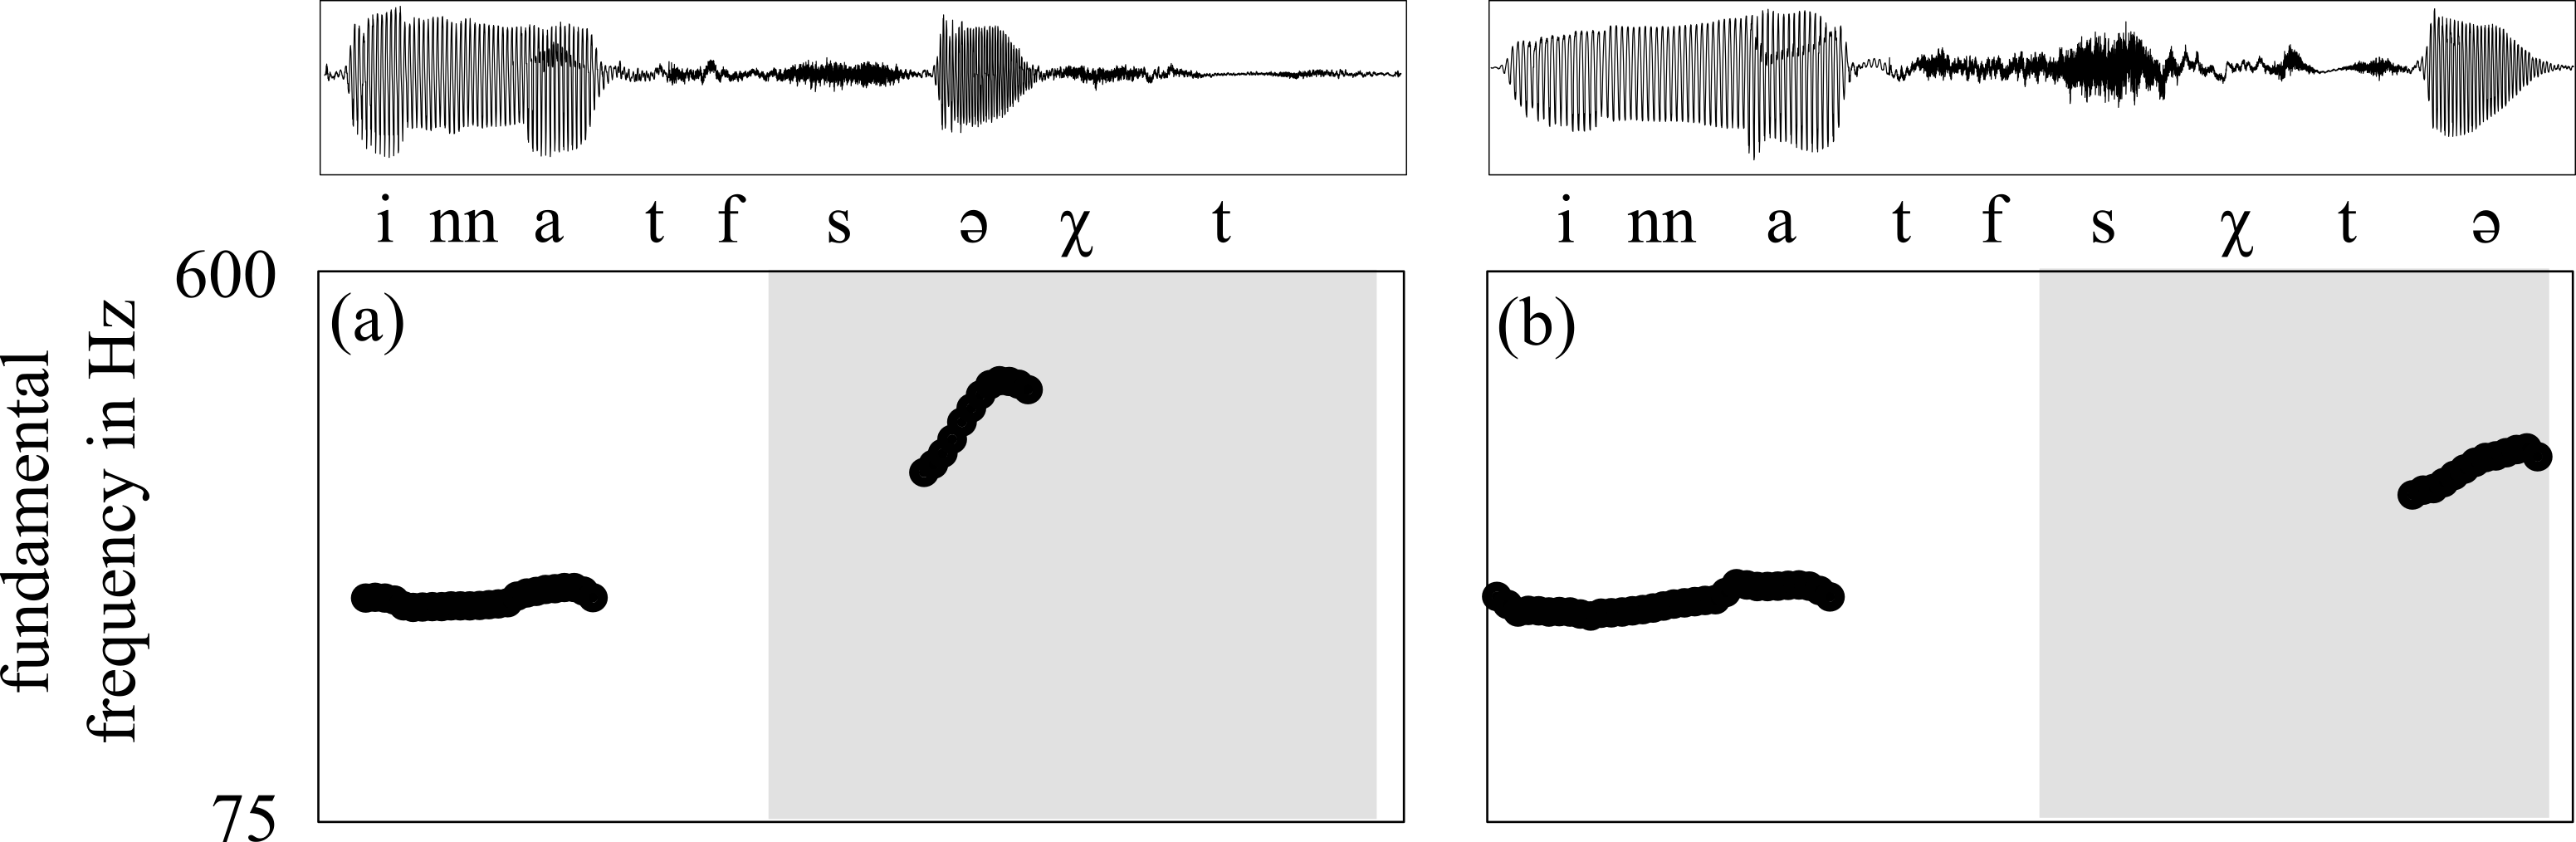
\includegraphics[width=1\textwidth]{figures/Figure_6_7_tfsxt.png}
  \caption{Representative waveforms and f0 contours of echo questions containing phonologically voiceless target words in phrase-final position (target word /tfsχt/). (a) illustrates schwa in word-medial position and (b) illustrates schwa in word-final position. Final syllables are highlighted in grey.}
   \label{fig:6.7}
   \end{figure}
   
  \begin{figure}
   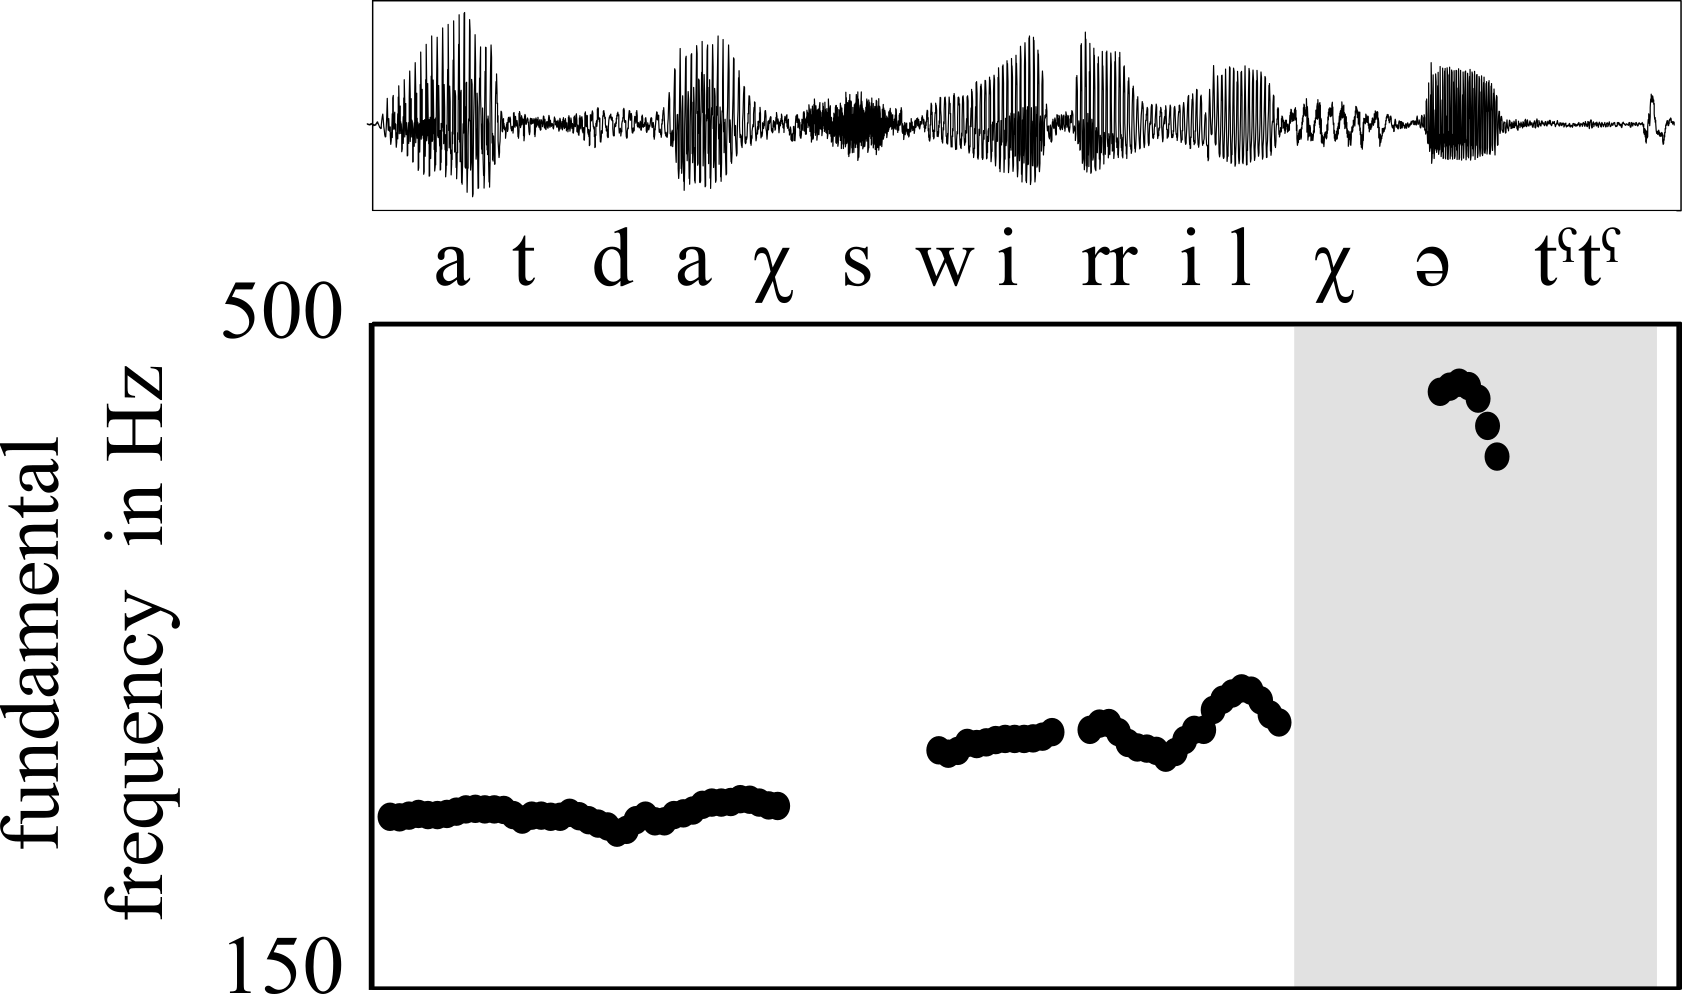
\includegraphics[width=0.6\textwidth]{figures/Figure_6_8.png}
  \caption{Representative waveform and f0 contour of the declarative question /ad d daχ swirriχ lxtˁtˁ/ ‘I make the line go back?’ The final syllable is highlighted in grey.}
   \label{fig:6.8}
   \end{figure}
   
\newpage    
Before considering the quantitative aspects of this phenomenon, it is important to note that schwas carrying functionally relevant pitch movements are not restricted to elicited speech but they are also found in natural data. \figref{fig:6.8} illustrates a declarative question ending on voiceless segments. A schwa is found between /χ/ and /tˁtˁ/ and it carries high pitch. Such patterns are quite frequently observed, especially in phrase-final position of phrases marked for non-finality.   
   
\subsubsection{Exploratory analysis}
Random forest analyses enable us to identify which factors  contribute to predicting the presence vs. absence of schwa independently, thus, accounting for collinearity between factors. The following factors were included in the analysis: factors capturing idiosyncratic properties of speakers in addition to speaker origin and speaker gender, factors capturing idiosyncratic properties of words, a factor capturing differences in sentence modality (y/n question, echo question, statement, negative statement), and a factor capturing the position of the word within the utterance (phrase medial vs. phrase final). \figref{fig:6.9} displays the variable importance estimated by the model, i.e. the relative relevance of the factors. The factors are ranked from top to bottom by importance. As can be seen, all of the factors capture some of the variance. Tables \figref{tab:6.3} and \figref{tab:6.4} display the observed proportions with respect to the relevant factors.

  \begin{figure}
   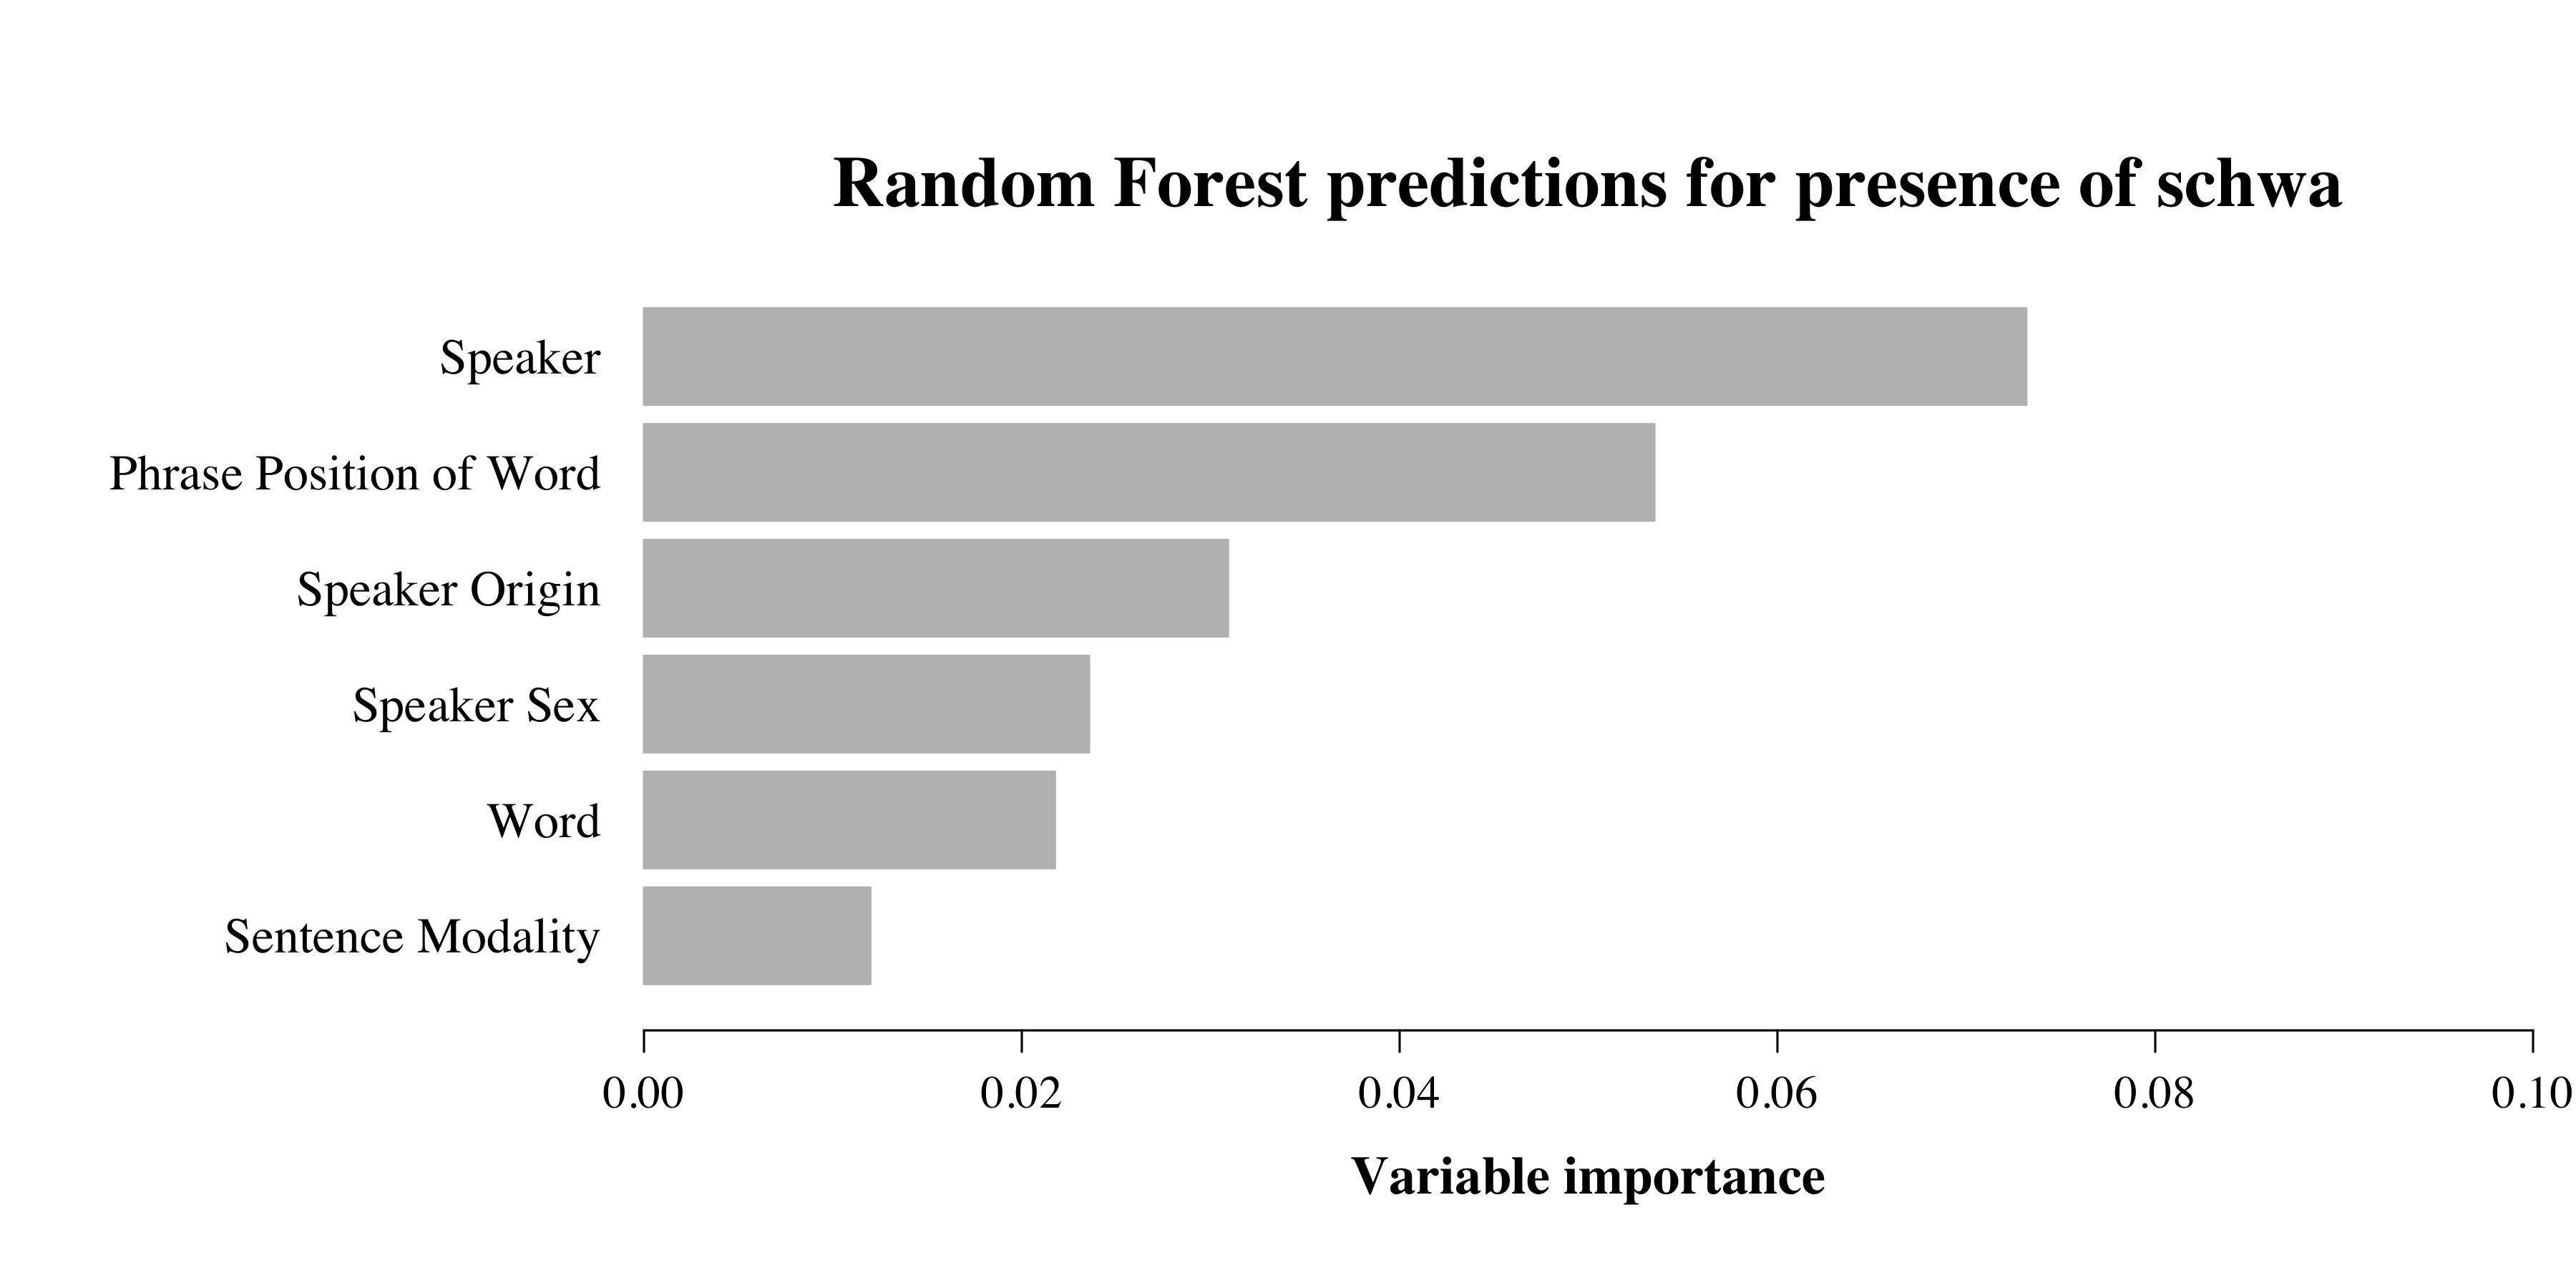
\includegraphics[width=1\textwidth]{figures/Figure_6_9.png}
  \caption{Variable importance for the prediction of schwa presence generated by the random forest analysis for all utterances containing phonologically voiceless words.}
   \label{fig:6.9}
   \end{figure}

\begin{table}[htbp]
    \begin{tabular}{cccc}
\lsptoprule    
    \multirow{2}[3]{*}{\textbf{Speaker}} & \multirow{2}[3]{*}{\textbf{Schwa}} & \multicolumn{2}{c}{\textbf{Position in Word}} \\
\cmidrule{3-4} & & \textbf{CəC} & \textbf{Cə\#} \\
    \midrule
    F1 (Agadir) &          0.54    &          1.00    &              -      \\
    F2 (Taroudant) &          0.76    &          0.98    &           0.02    \\
    F3 (Agadir) &          0.97    &          0.98    &           0.02    \\
    F4 (Agadir) &          0.75    &          0.07    &           0.93    \\
    F5 (Anti-Atlas) &          0.87    &          1.00    &              -      \\
    \midrule
    M1 (Agadir) &          0.44    &          0.04    &           0.96    \\
    M2 (Taroudant) &          0.70    &          1.00    &              -      \\
    M3 (Anti-Atlas) &              -      &              -      &              -      \\
    M4 (Anti-Atlas) &              -      &              -      &              -      \\
    M5 (Agadir) &          0.48    &          1.00    &              -      \\
    \midrule
    \lspbottomrule
    \textbf{mean} & \textbf{         0.57   } & \textbf{         0.67   } & \textbf{          0.33   } \\
    \end{tabular}
    \caption{Mean proportions of productions exhibiting schwa averaged over words. The proportion of word-medial (CəC) and word-final schwa (Cə\#) is given in relative terms.}
  \label{tab:6.3}
\end{table}

\begin{table}[htbp]
  
    \begin{tabular}{cccc}
    \lsptoprule
    \multirow{2}[3]{*}{\textbf{Word}} & \multirow{2}[3]{*}{\textbf{Schwa}} & \multicolumn{2}{c}{\textbf{Position in Word}} \\
\cmidrule{3-4}  & & \textbf{CəC} & \textbf{Cə\#} \\
    \midrule
    ʃʃ    &          0.20    &              -      &          1.00    \\
    ʃtf   &          0.56    &          0.60    &          0.40    \\
    ftχ   &          0.50    &          0.44    &          0.56    \\
    tʃtft &          0.67    &          0.74    &          0.26    \\
    tfss  &          0.42    &          0.38    &          0.63    \\
    tfsχt &          0.70    &          0.71    &          0.29    \\
    tkʃf  &          0.54    &          0.66    &          0.34    \\
    tsxf  &          0.53    &          0.68    &          0.32    \\
    \midrule
    \textbf{mean} & \textbf{         0.57   } & \textbf{         0.67   } & \textbf{         0.33   } \\
    \lspbottomrule
    \end{tabular}
\caption{Mean proportions of productions exhibiting schwa averaged over speakers. The proportion of word-medial (CəC) and word-final schwa (Cə\#) is given in relative terms.}
  \label{tab:6.4}
\end{table}

The factor capturing idiosyncratic properties of the speakers themselves is the highest ranked predictor. There are two speakers that showed no schwa (M3 and M4) while F3, for example, almost always produced a schwa. Additionally, both the area in which the speaker was brought up and the gender of the speaker explain additional variance. There is a general trend for speakers coming from rural areas (Anti-Atlas) to produce less schwa (33\%) than those from urban areas (Agadir and Taroudant: 67\%). Furthermore, women produce generally more schwa (77\%) than men (36\%) (cf. \tabref{tab:6.3}). According to the random forest analysis, these factors explain observed variability independently of each other. The other source of potential idiosyncratic variability is the lexical word in which schwa surfaces. As can be seen in \tabref{tab:6.4}, there are large differences across words. Some words are produced with schwa in two thirds of all productions (/tʃtft/ and /tfsχt/), while others are barely produced with schwa (e.g. /ʃʃ/).

Apart from idiosyncratic factors of speakers and words, phrase position has been estimated to have the second highest variable importance. Target words in phrase-final position exhibit schwa more often (64\%) than target words in phrase-medial position (41\%). This pattern is consistent across speakers, words, and sentence modalities. This proportional trend is reflected by durational patterns with schwa being generally longer in phrase-final words than in phrase-medial words. (cf. \tabref{tab:6.5}).

\begin{table}[htbp]
  \fittable{
    \begin{tabular}{cccccc}
    \lsptoprule
    \multirow{2}[1]{*}{\textbf{Sentence Modality}} & \multirow{2}[1]{*}{\textbf{Phrase Position}} & \multicolumn{2}{c}{\multirow{2}[1]{*}{\textbf{Schwa Presence}}} & \multicolumn{2}{c}{\multirow{2}[1]{*}{\textbf{Schwa Duration}}} \\
          &       & \multicolumn{2}{c}{} & \multicolumn{2}{c}{} \\
    \midrule
    \multirow{2}[4]{*}{Y/N Question} & Medial & 0.43  & \multirow{2}[4]{*}{0.66} & 50 (12) & \multirow{2}[4]{*}{82 (30)} \\
\cmidrule{2-3}\cmidrule{5-5}          & Final & 0.78  &       & 91 (28) &  \\
    \midrule
    \multirow{2}[4]{*}{Echo Question} & Medial & 0.33  & \multirow{2}[4]{*}{0.55} & 50 (12) & \multirow{2}[4]{*}{83 (27)} \\
\cmidrule{2-3}\cmidrule{5-5}          & Final & 0.64  &       & 89 (24) &  \\
    \midrule
    \multirow{2}[4]{*}{Contrastive Statement} & Medial & 0.67  & \multirow{2}[4]{*}{0.73} & 62 (4) & \multirow{2}[4]{*}{81 (22)} \\
\cmidrule{2-3}\cmidrule{5-5}          & Final & 0.76  &       & 88 (21) &  \\
    \midrule
    \multirow{2}[4]{*}{Negative Statement} & Medial & 0.34  & \multirow{2}[4]{*}{0.51} & 55 (13) & \multirow{2}[4]{*}{78 (2)} \\
\cmidrule{2-3}\cmidrule{5-5}          & Final & 0.57  &       & 82 (19) &  \\
    \lspbottomrule
    \end{tabular}
    }
      \caption{Mean proportions of schwa and duration of schwa (in ms) for sentence modality and phrase position of the word it occurred in averaged over words and speakers.}
  \label{tab:6.5}
\end{table}

Even though it is the least important variable in the model, sentence modality is estimated to independently explain some of the variance. Contrastive statements exhibit the highest proportion of schwa, followed by questions, and negative statements. 

Having explored potential aspects affecting the presence of schwa, we now turn to the curious divergence between schwa in word-medial and word-final position. The same factors used for the random forest analysis above were included predicting the position of schwa within the word (cf. \figref{fig:6.10}). 

  \begin{figure}
   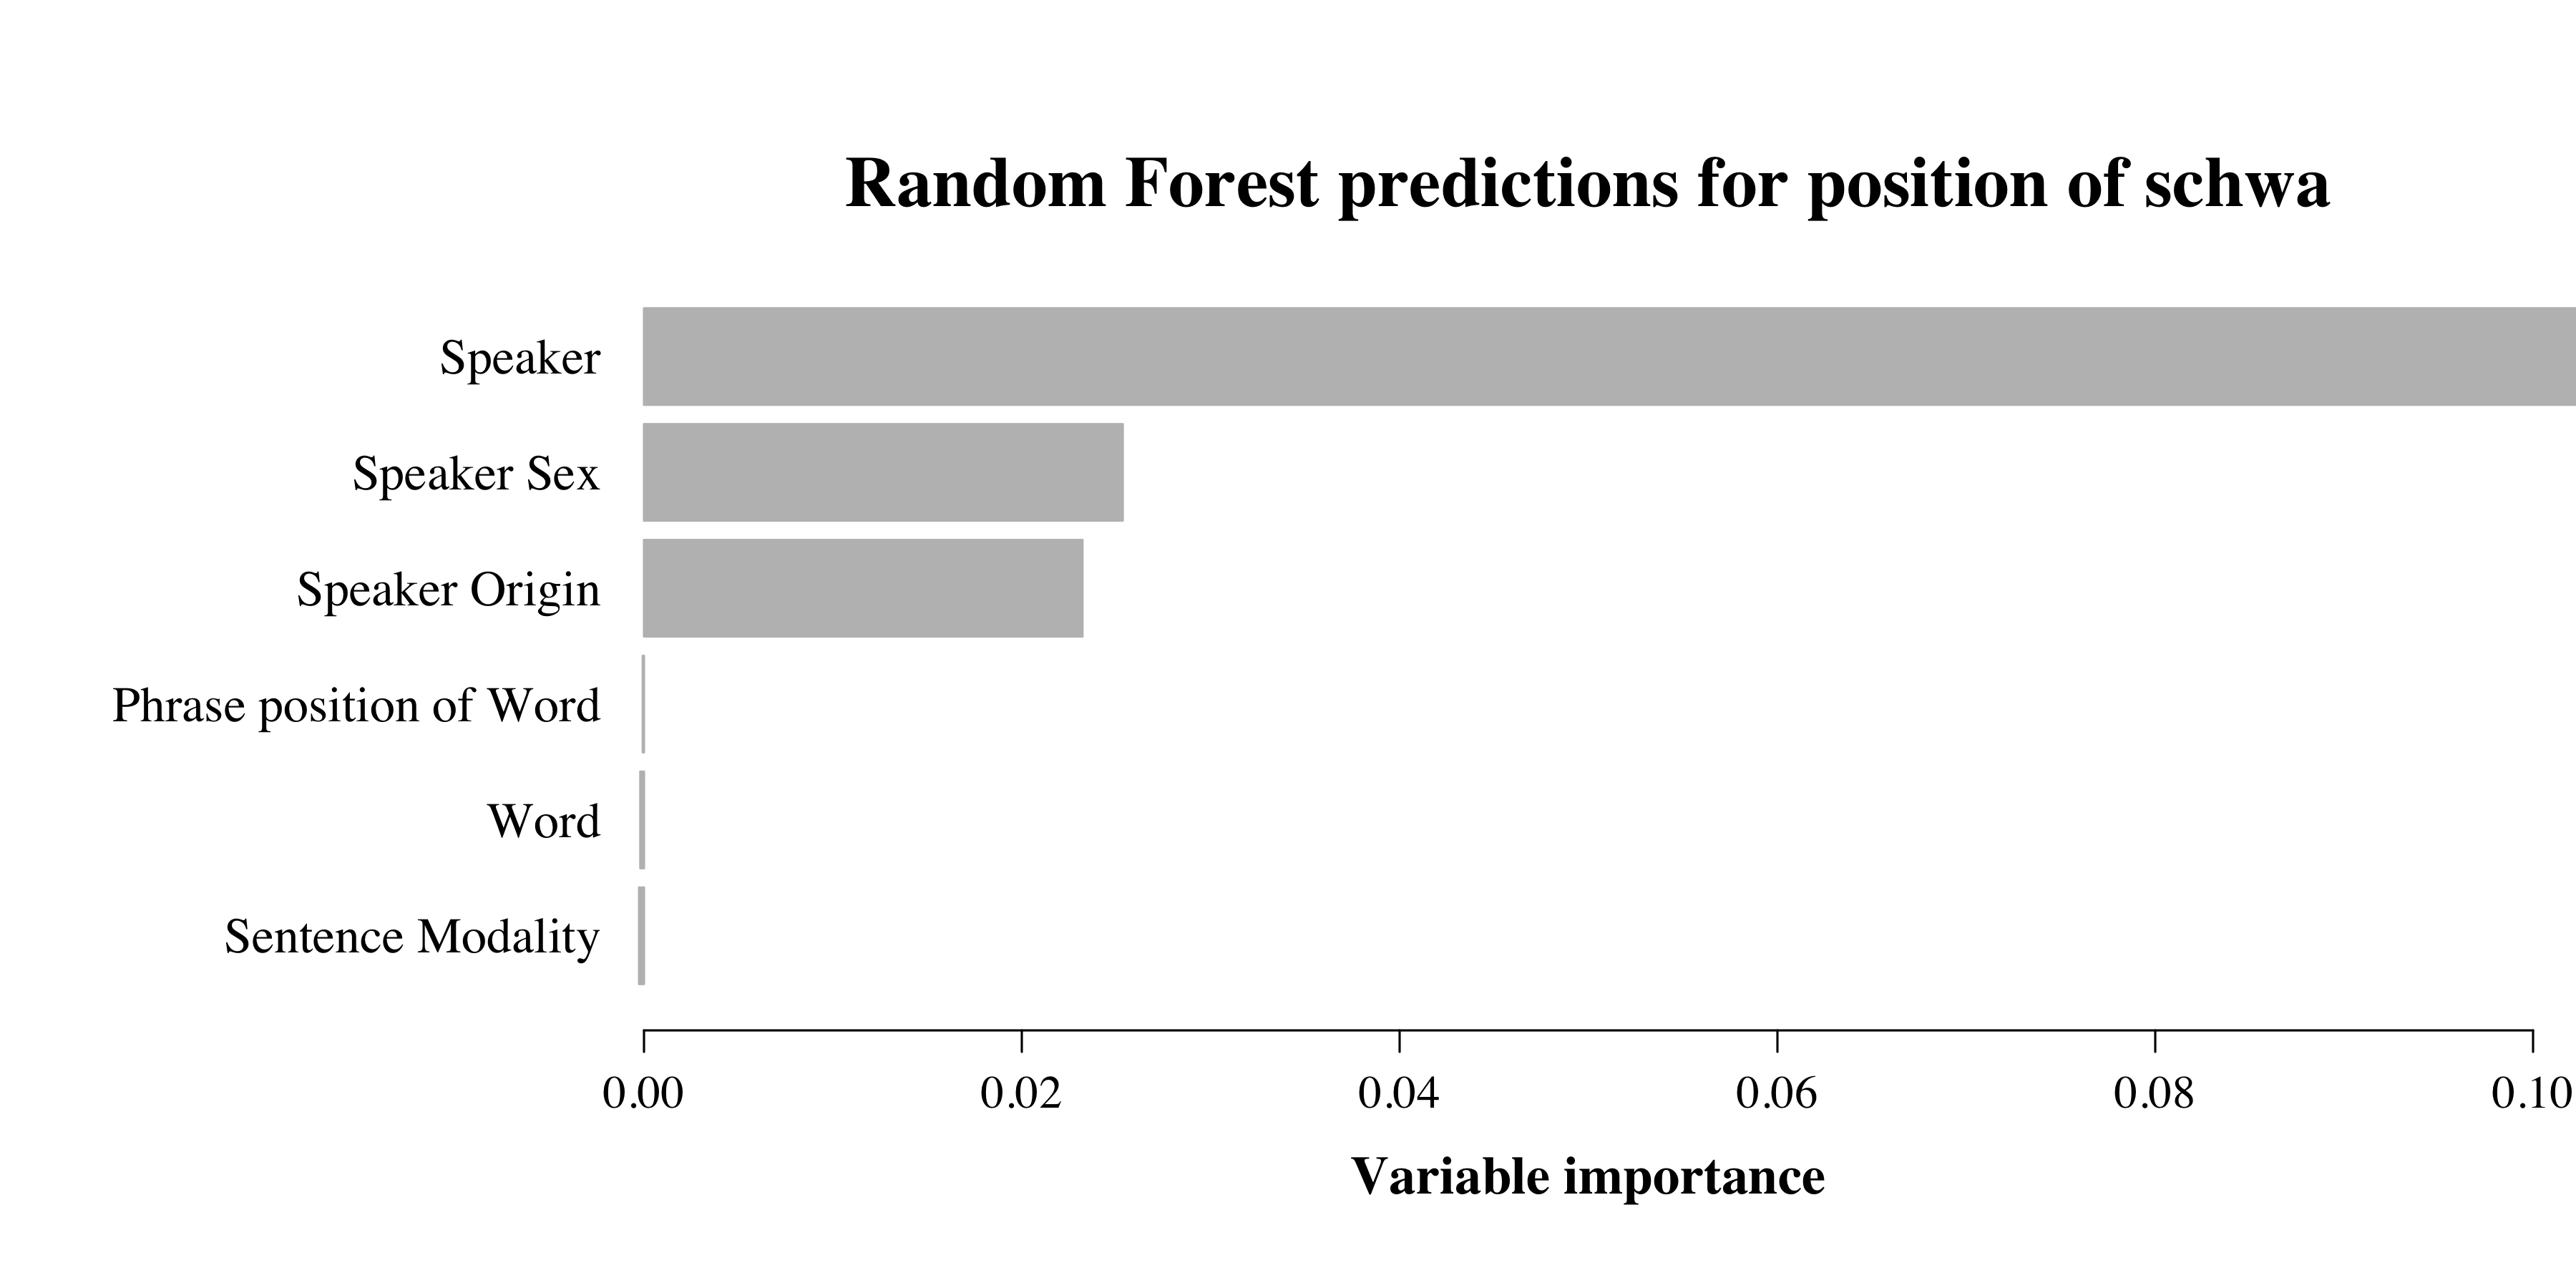
\includegraphics[width=1\textwidth]{figures/Figure_6_10.png}
  \caption{Variable importance measure for the position of schwa within the word generated by the random forest analysis for all utterances containing schwa in phonologically voiceless words.}
   \label{fig:6.10}
   \end{figure}

This model estimates that speaker information is by far the most important predictor. Apart from some indications of speaker gender and speaker origin playing a role (women = 18\% word-final schwa, men = 68\%; Agadir = 33\% word-final schwa, Taroudant = 50\%, Anti-Atlas = 0\%), most variance is explained by speaker specific behaviour irrespective of gender and origin. Other linguistic factors appear to have no impact on the position of schwa within the word.

\subsubsection{Summary}
To sum up, the present exploration has revealed a large number of schwa in phonologically voiceless environments. Schwa appears in two particular positions in the word. It is either between the onset and nucleus of the final syllable (e.g. [tkʃəf], [tsχəf̩]) or in word-final position (e.g. [tkʃfə], [tsχfə]). As opposed to earlier studies (that used speakers who had lived in France for a significant amount of time), schwa is not found between syllables or between the nucleus and the coda (\citealt{Grice.etal2011,Grice.etal2015tash}). This rather strict appearance of schwa in a specific structural position, irrespective of the supralaryngeal properties of the consonantal environment, is remarkable and should be considered when evaluating the status of schwa in Tashlhiyt (also highlighted by \citealt{GordonNafi2012}). When schwa is present, it carries characteristic aspects of the tonal contour, e.g. parts of the rise-fall in questions and contrastive statements. This is the case regardless of the position of schwa, i.e. the same characteristic aspect of the contour is realised on word-medial and on word-final schwas. 

\newpage
Explorative statistical analyses reveal that the presence of schwa was to some degree predictable from the phrase position of the word in which schwa surfaced (phrase medial vs. phrase final) and sentence modality of the utterance. In addition to these linguistic factors, both the presence of schwas and the position of schwa within the word are strongly affected by properties of the speaker sample. In addition to idiosyncratic properties of each individual speaker, speaker origin, and speaker gender played a role. 

\section{The status of schwa revisited}\label{sec:6.5}
\subsection{Schwa as a sociolinguistic marker}
Both the presence of schwa and the position of schwa within the word is prone to a large amount of both within and across speaker variation. This variation is to some degree accountable by demographic factors like the area in which the speaker was brought up and his / her gender. This is in line with the discussion of the sociolinguistic dimension of schwa by \citet{Boukous2012}. He recognised that in urban areas, children are more likely to produce a schwa between consonants, which, according to Boukous, occupies the syllable nucleus position. He attributes this feature to the strong influence of Moroccan Arabic on Tashlhiyt. \is{vowel insertion} 

\begin{quote}
 
Nous remarquons que dans les formes réalisées par les sujets appartenant au groupe des enfants ruraux, les syllabes n'ont pas de noyau vocalique alors que dans celles performées par les enfants citadins il y a insertion d'une voyelle de type schwa (ə) pour constituer le noyau de la syllabe. Cette habitude articulatoire est probablement acquise avec l'arabe dialectal car l'insertion du schwa correspond à une nécessité de la phonotaxe de l'arabe marocain […].ˮ (\citealt[83]{Boukous2012})\footnote{“We notice that in the forms realised by the subjects belonging to the group of rural children, the syllables do not have a vocalic nucleus whereas in the ones performed by the urban group of children there is an insertion of a schwa type vowel (ə) forming the nucleus of the syllable. This articulatory habit is probably acquired with dialectal Arabic because the insertion of the schwa corresponds to a phonotactic requirement of Moroccan Arabic […] (my own translation)}
\end{quote}

Boukous already acknowledges a potential phonological status of schwa in the speech of Tashlhiyt speakers in urban areas. However, instead of being a native phenomenon, it is attributed to the contact with Moroccan Arabic. In addition to the three cardinal vowels /i, a, u/, Moroccan Arabic has a phonological schwa, the position of which can be distinctive (compare /həbs/ ‘prison’ and /hbəs/ ‘imprison’). This stands in contrast to Tashlhiyt, which does not exhibit such minimal pairs. Therefore, one should exercise caution when attributing a phonological status to schwa in Tashlhiyt simply due to the assumption that it is borrowed from a language in which schwa is a phonological element.\is{vowel insertion}  

While Boukous does not explicitly discuss the position of schwa within the word, Ridouane (2008: 337) attributes word-medial schwas in his data to language contact with Moroccan Arabic. In light of its sociolinguistic context, it might be objected that the observed variability in the present production data is due to a heterogeneous sample, i.e. speakers from different subvarieties of Tashlhiyt (see \tabref{tab:6.3} and Appendix A2.2 for an overview of speaker origins). In defence of considering the recorded speakers together as representing a single variety (see also \citealt{Bruggeman.etal2017}) one could argue that differences between speakers from geographically distant areas do not supersede the differences between speakers with the same birthplace. Speakers who grew up in Agadir do not behave more uniformly than any other grouping of speakers. Thus, it can be concluded that the observed variability is not solely caused by the heterogeneous sample. Other demographic or sociolinguistic properties of the speakers beyond the present investigation might account for these different production patterns.\is{vowel insertion} 

It is noteworthy that this potential contact phenomenon goes against other sociolinguistic trends. Tashlhiyt speakers (at least the educated speakers that were recorded in the present sample) are highly self-conscious of schwa not being a phoneme in Tashlhiyt. However, they are clearly aware of schwa being a phonological element in other Berber varieties and Moroccan Arabic. In other words, Tashlhiyt speakers have a high awareness of schwa being a linguistic feature that distinguishes their own language from other languages in the area. Despite this awareness, they do produce schwa in the majority of utterances. This tension between language contact and language identity may cause a high degree of variability within and across studies and might be one of the reasons why the literature was unable to settle on any consensus regarding the status of schwa.

\subsection{Schwa as reflecting gestural reorganisation}
Irrespective of schwa being to some degree dependent on speaker-specific properties, schwa is determined by prosodic and intonational properties of the utterance. Schwa occurs more often in words in phrase-final position than in phrase-medial position, irrespective of sentence modality. This is in line with \citet{Ridouane2008} reporting on more schwa in words produced in isolation than in words inserted in carrier sentences with the target word in phrase-medial position. Additionally, looking at schwa occurrences in phrase-medial words only, one sentence modality stands out: words in contrastive statements exhibit a substantially higher proportion of schwa (67\%) than questions (43/33\%) and negative assertions (34\%) (cf. \tabref{tab:6.4}). Questions are characterised by a pitch peak at the right edge of the phrase. Negations are characterised by a pitch peak at the beginning of the utterance (on /ur-/, the negative marker). In both questions and negations, there is no tonal event on the phrase-medial target word. As opposed to questions and negative assertions, contrastive statements are characterised by a tonal event on the target word in phrase-medial position. This suggests a correlation between the proportion of observed schwas and the occurrence of communicatively relevant tonal events. This correlation can be accounted for by dynamics of speech production. It is well known that elements in certain prosodically privileged position are spatio-temporally adjusted (introduced in Chapter 2 and 5). This adjustment refers either to edge-induced strengthening, e.g. final lengthening, or to prominence-induced strengthening.\is{gestural coordination}\is{vowel insertion} 

For example, it has been shown that the syllable rhyme is longer in final position of prosodic constituents than in non-final position for English (e.g. \citealt{TurkShattuck2007}). In addition to temporal adjustments, elements in phrase-final position have been shown to exhibit increased jaw movement duration and decreased velocity of oral closing gestures (\citealt{BeckmanEdwards1990,Edwards.etal1991}). \il{English} 

\largerpage
Similarly, articulatory gestures may be adjusted due to prominence-induced strengthening. In many languages, certain elements of the utterances can be emphasised by intonational events. In languages with lexical word stress, pragmatically highlighted words can co-occur with a pitch accent. Research conducted mainly on languages that exhibit such pitch accents (e.g. English, French, Italian, and German) reports that the co-occurrence of a pitch accent with a syllable results in temporal and spatial expansion of the articulatory gestures involved.\citet{ChoKeating2009} found longer durations for /n/ and higher burst intensities for the alveolar plosive /t/ in accented position. Alongside, longer vowels, \citet{ChoMcQueen2005} found evidence for a strengthening of fricatives and stops in accented syllables in Dutch (e.g. closure / frication duration, voicing duration, VOT). With respect to spatial properties, vowels tend to be hyperarticulated in accented position. For example, in his work on English, \citet{Cho2005} showed that vowels in accented position were articulated with longer jaw opening gestures than respective vowels of unaccented syllables. He further showed that /a/ is consistently lowered and /i/ is consistently fronted when accented. Similarly, \citet{Harrington.etal2000} showed that English high vowels are generally raised when accented.\is{gestural coordination} \il{English}\il{French}\il{Italian}\il{German}\il{Dutch}
  
While not explicitly tested for in the present study,\footnote{Note that spatio-temporal asymmetries as a function of co-occurrence with a tonal event are empirically difficult to evaluate in Tashlhiyt, since the co-occurrence of a tone with a specific syllable is not deterministically predictable. In both \citet{Grice.etal2015tash} and the present production corpus, pitch peaks on the penult and the final syllable were distributed in a very unbalanced way making a statistical assessment based on such a small sample impossible.} several indirect arguments indicate that there are similar spatio-temporal adjustments of segments as a function of their co-occurrence with a tonal event. First, several phoneticians working with the data sets presented here (the author, Grice, Bruggeman, Ridouane) perceived the syllable the tone co-occurs with as more prominent than other syllables. Of course, one has to exercise great caution when interpreting such impressionistic observations made by analysts speaking languages that have prominence-lending pitch accents.

Second, \citet{GordonNafi2012} found evidence for duration and intensity asymmetries across syllables as a function of the co-occurrence with a tone. As has been argued in Chapter 4, these asymmetries cannot be attributed to lexical stress, but can be related to the postlexical tonal events with which the segmental material co-occurs.\is{word stress} 

Third, there is some anecdotal evidence that a vowel is spatio-temporally extended when it co-occurs with a pitch peak. \citet{Grice.etal2011} investigated the nature and distribution of phrase-medial pitch peaks in contrastive sentences for three Tashlhiyt speakers (similar to Chapter 5). In line with the findings reported on here, the contrasted element co-occurred with a rise-fall in pitch. When there was no sonorant available, the authors obtained highly variable tonal placement. They observed patterns equivalent to the anticipated tone pattern and the tone on schwa pattern discussed in section \sectref{sec:6.2}. \citegen{Grice.etal2011} data was recorded for an independent articulatory experiment (\citealt{Hermes.etal2011}). This allowed \citet{Diercks2011} to take a closer look at both acoustic and articulatory patterns of segments as a function of their co-occurrence with the pitch peak. Diercks looked at the productions of one speaker who revealed a high degree of variation between the anticipated tone pattern and the tone on schwa pattern. Acoustic analyses revealed that the word /inna/ was longer and that the vowel /a/ exhibited lower F1 values when co-occurring with the pitch peak (\figref{fig:6.11}, left panel). The acoustic results were reflected in the kinematic data. When /a/ co-occurred with the pitch peak, the tongue body was lower than when the vowel did not occur with the pitch peak (cf. \figref{fig:6.11}, right panel).

  \begin{figure}
   
   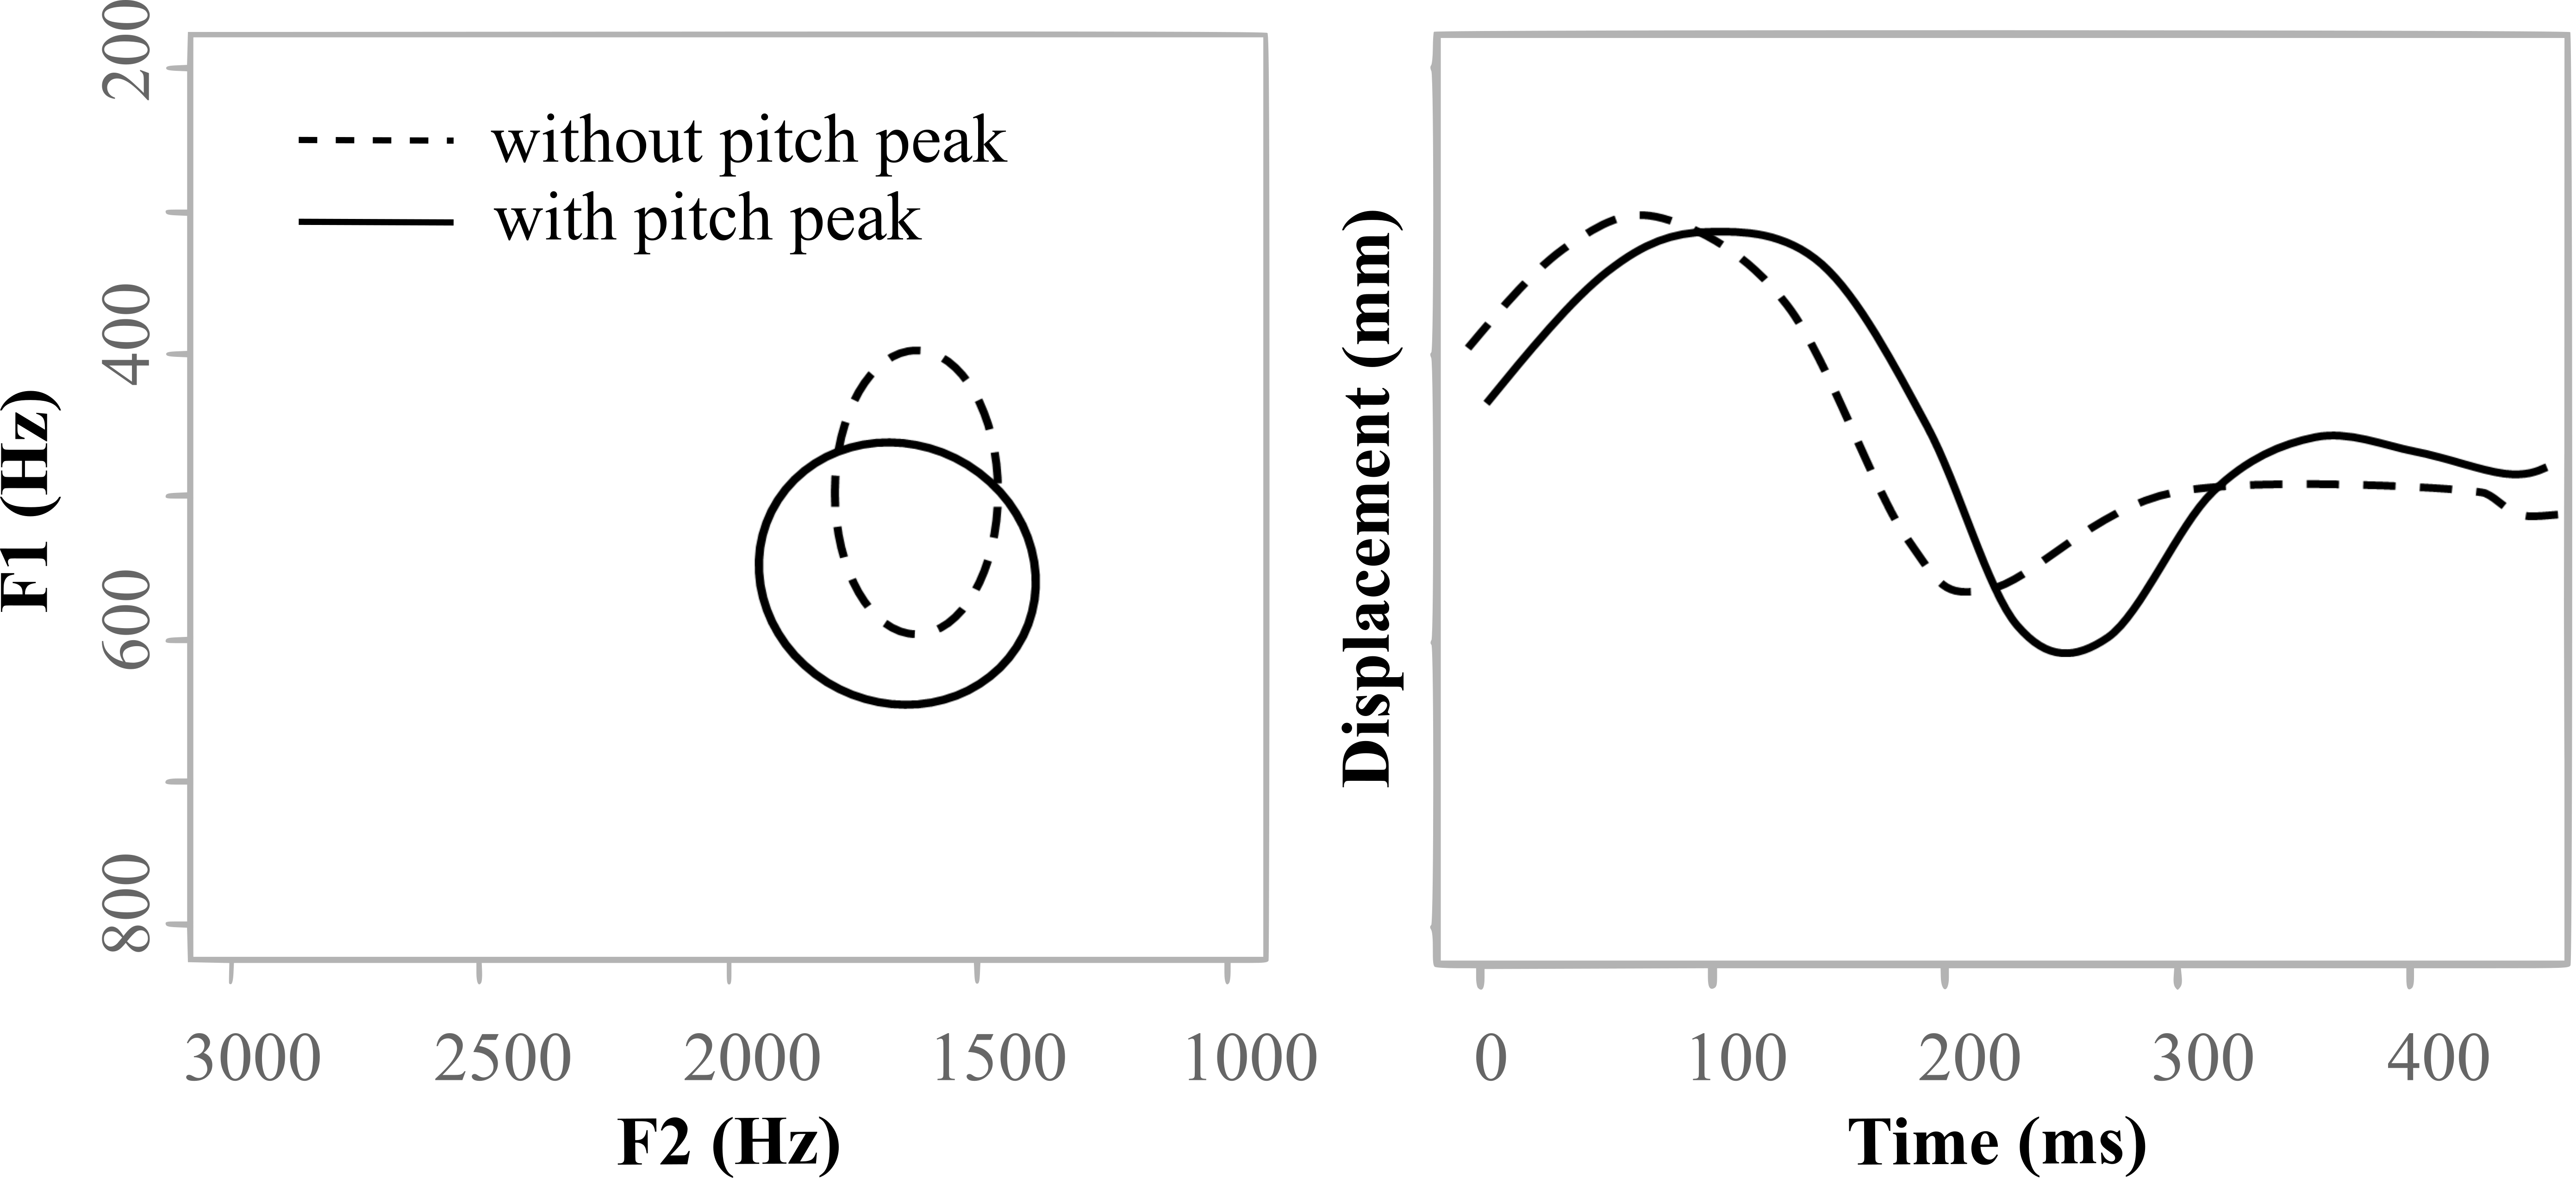
\includegraphics[width=1\textwidth]{figures/Figure_6_11_Diercks.png}
  \caption{Left panel displays F1 and F2 of /a/ in /inna/ dependent on the presence of the pitch peak. Right panel displays averaged vertical trajectories of the tongue body in /inna/. Figures taken from \citet{Diercks2011}. Note: Diercks does not provide a y-axis for the displacement values.}
   \label{fig:6.11}
   \end{figure}

    \largerpage
In line with the literature on prominence-induced strengthening (e.g. \citealt{Harrington.etal2000,ChoKeating2009,MueckeGrice2014}), the rise-fall in Tashlhiyt caused spatio-temporal expansion of the segments it co-occurred with. Here the open vowel /a/ is lowered.

Both edge-induced strengthening and prominence-induced strengthening can be conceptualised as a local slowing down of articulatory gestures resulting in less gestural overlap and more precise achievement of articulatory targets (\citealt{ByrdSaltzman2003,Saltzman2008}). This slowing down mechanism may explain the phrase-position dependent presence of schwa in Tashlhiyt. In both phrasal positions in which less gestural overlap is expected (phrase-final position and in those positions where a tonal event occurs phrase medially), we observe an increased proportion of schwa and an increased duration of schwa when it is present.\is{gestural coordination} 

Prosodically triggered gestural adjustments may not only affect oral gestures, but laryngeal gestures, too. According to \citet{Ridouane2007lar}, voiceless consonant clusters in Tashlhiyt have to be considered as sequences of multiple glottal opening gestures. Using transillumination, they measured the degree of glottal adduction during voiceless consonant clusters. They showed that in words made up of voiceless obstruents only, the glottis does not simply remain open. The glottal aperture is modulated by the segments with which it co-occurs. This is interpreted as evidence for separate glottal opening gestures that are coupled to supralaryngeal gestures. Given these findings, a slowing down of the articulation might result in less overlap of both oral and glottal opening gestures. If glottal opening gestures are sufficiently apart, glottal adduction can occur. This, in turn, would lead to an articulatory configuration that gives rise to a vowel-like element, i.e. an open oral transition accompanied by glottal adduction (\citealt{Goldstein2011,Goldstein2014}).\is{gestural coordination} 

Based on these mechanisms, a voiced interval within a voiceless cluster could be attributed to a gestural reorganisation reflecting a prosodically triggered adjustment. The proposed interpretation can be considered a purely phonetic one, i.e. schwa is an artefact of the dynamic interaction of individual articulatory gestures and higher prosodic relationships. It is thus highly compatible with the transitional vocoid account. This articulatory model might even be able to account for word-final schwas: if the release of the final consonant is slowed down and remains active beyond the glottal opening gesture of the consonant, the glottis will achieve its default position in speech (adducted) before the end of the release, resulting in a voiced interval (\citealt{Goldstein2014}).\footnote{It is important to note that this account is speculative and based on indirect evidence, since laryngeal gestures were not investigated directly.}\is{gestural coordination} 

Importantly, the discussed model and its articulatory predictions are not only interpretable in terms of the transitional vocoid account; they are also compatible with Coleman’s epenthetic vowel account. The latter explicitly assumes that a phonological schwa can be obscured by surrounding articulatory gestures. Its phonetic variability would be accounted for by the degree of gestural overlap as a function of prosodic position. According to Coleman, the assumed underlying schwa in the first syllable in /təs.ti/ does not surface acoustically because it is completely overlapped by the surrounding consonantal gestures. Similarly, one could argue that schwa usually does not surface in voiceless clusters because the glottal opening gestures of the surrounding consonants overlap heavily, which disables the voicing of schwa to surface. However, in certain prosodic positions these glottal opening gestures are pulled apart, enabling schwa to surface acoustically. The epenthetic vowel account could thus capture the asymmetries found in the present corpus just as well as the transitional vocoid account.\is{vowel insertion}\is{gestural coordination} 

Neither the original epenthetic vowel account nor the original transitional vocoid account were able to explain the observed schwa asymmetries related to the phrasal context (\citealt{Ridouane2008,GordonNafi2012}; the present study). However, some of those anomalies can be accounted for with the presented gestural organisation model taking into account that articulatory gestures are modulated by prosodic and intonational factors (\citealt{ByrdSaltzman2003,Saltzman2008,Goldstein2014}). This model is compatible with schwa in voiceless environments. Even though schwa is traditionally not expected to occur in voiceless clusters, gestural reorganisation in prosodically privileged positions may lead to an underlap of glottal opening gestures and, in turn, may result in voicing in both word-internal and word-final position. This account, however, does not provide conclusive evidence in favour of either the epenthetic vowel account or the transitional vocoid account. To a certain degree, both accounts are compatible with the idea of gestural underlap.  \is{gestural coordination} 

Even though prosodically triggered gestural reorganisation in combination with both the epenthetic vowel account and the transitional vocoid account may explain some observations, there remain unresolved issues: neither can explain why there is a robust alternation between word-medial and word-final schwa. Crucially, these schwa locations are mutually exclusive, i.e. when a schwa occurs in word-medial position, it does not occur in word-final position and vice versa. Moreover, throughout the reading experiment, speakers use either one pattern or the other with very few exceptions. The epenthetic vowel account would have to assume that speakers differ with respect to their lexical representations. For example, while speaker F1’s production [tkʃəf] would be a reflection of /tək.ʃəf/, speaker F4’s production [tkʃfə] would be a reflection of /təkʃ.fə/. The alternation in this case would be at the lexical level of phonological representation rather than at the level of phonetic instantiation.\is{vowel insertion} 

Alternatively, this alternation could be due to variable gestural reorganisation. Similar to discrete tonal alignment patterns observed in words with more than one sonorant nucleus (see Chapter 5), speakers might probabilistically produce schwa in either word-medial or word-final position dependent on sentence modality. However, individual speakers have a clear preference for either one or the other position. As the random forest analysis suggests, sentence modality does not have an impact on the choice between the two patterns at all. This alternation, therefore, is fundamentally different from the one observed for tonal placement in words containing vowels and sonorant consonants, where there is more within-speaker variation.\is{vowel insertion} 

The production data presented in section \sectref{sec:6.3} suggest that the alternation between word-medial and word-final schwa may be due to demographic characteristics such as gender and place of upbringing. This suggests a sociolinguistic component to schwa (see also \citealt{Boukous2012}) which is not covered by any of the above discussed accounts.\is{vowel insertion} 

In addition to speaker variability, proponents of the transitional vocoid account have criticised the epenthetic vowel account for predicting the occurrence of more schwas than actually attested as well as the occurrences of schwas in positions where they are not attested at all (see \sectref{sec:6.3}). However, the transitional vocoid account has also problems accounting for distributional facts. In the present study, word-medial schwa is always found between the onset and the nucleus consonant of the final syllable (see also \citealt{GordonNafi2012}). This preference for a particular structural position does not follow from the transitional vocoid account, which assumes that the presence of schwa is predominantly determined by laryngeal and supralaryngeal properties. In the epenthetic vowel account, schwa is considered a phonological element that occupies an empty syllable nucleus position in syllables with no lexical vowels. This model predicts an epenthetic schwa in exactly this structural position, between the onset and the nucleus (according to Dell and Elmedlaoui’s syllabification algorithm). However, one may ask the question as to why schwa in the present data only appears in the final syllable (e.g. /tk.ʃəf/) and not in the penult (e.g. /tək.ʃf/) or in both syllables (e.g. /tək.ʃəf/). \is{vowel insertion} 

\subsection{Schwa as a prosodic marker}
In the following, we introduce a way to resolve some of the conflicts between these competing accounts: Tashlhiyt may exhibit two different types of schwa: one schwa is merely a transitional vocoid with no relevance for any phonological component whatsoever; the other is at least relevant for the alignment of intonational tones (\citealt{GordonNafi2012}). This dichotomy roughly matches the typology of inserted vowels proposed by \citet{Hall2006}. She has argued that there are two distinct kinds of inserted vowels (see also \citealt{Harms1976,Levin1987,Warner.etal2001,Silverman2011}). On the one hand, there are intrusive (or excrescent) vocoids, i.e. phonetic transitions between two consonantal gestures that do not exhibit any phonological status and are thus invisible to the phonological system. On the other hand, there are epenthetic vowels, i.e. segments that have stable forms and distributions and are visible to the phonological system.\is{vowel insertion}\is{gestural coordination} 

Different types of schwa within the same language have been proposed for Ath-Sidhar Rifian, a variety of Tarifiyt Berber spoken in North-Eastern Morocco (\citealt{DellTangi1992,DE2002}). One type of schwa in Ath-Sidhar Rifian has to be considered a transitional vocoid. This vocoid is never observed between homorganic and voiceless consonants. The other type of schwa in Ath-Sidhar Rifian is conceived of as phonologically inserted in order to syllabify sequences of consonants, similar to Coleman’s proposal for Tashlhiyt. The position of such epenthetic vowels may be the only feature that distinguishes two words from each other. Moreover, they are not constrained by the consonantal environment, i.e. they can occur between homorganic and voiceless consonants. Thus, non-phonological transitional vocoids co-exist with phonological epenthetic schwas across varieties of Berber.\il{Berber (Tarifiyt)}

In Tashlhiyt, the presence and form of intrusive vocoids is predictable from the laryngeal and supralaryngeal consonantal environment, their presence does not add duration to the syllable, and they play no role in any aspect of the phonological system, including versification, morphological processes, and intonation (e.g. \citealt{DE2002,DE2008,Ridouane2008,RidouaneFougeron2011}). These transitional vocoids are illustrated in \figref{fig:6.2}, where there are clear instances of schwas in the target word. These elements, however, do not carry the expected tonal event. It is likely that instrumental studies on schwa such as \citet{RidouaneFougeron2011}, which led to convincing empirical arguments for the non-phonological status of schwa, investigated mainly these types of intrusive vocoids.\is{vowel insertion} 

In addition to intrusive vocoids, Tashlhiyt exhibits something that may fall under the umbrella term of an ‘epenthetic vowel’. To distinguish it terminologically from the elements referred to in the epenthetic vowel account, it is referred to as a ‘postlexically triggered epenthetic vowel’ (PTEV). Neither its form nor its presence is fully predictable from its consonantal environment. However, note that it is still determined by the consonantal environment to some degree. In the data presented here, there was no schwa in homorganic clusters and schwa did not break up geminate consonants. Despite this, the phonological system −at least the intonation system− does refer to it. The present corpus provides strong arguments for schwa being an element that bears functional load, i.e. it enables the production of a functionally relevant tonal movement. Moreover, a pitch peak before the target word is incompatible with a PTEV within the target word, indicating a strong relationship between the presence of the PTEV and the location of the tone. However, the PTEV cannot be an epenthetic vowel that is always eligible for tonal alignment; it is rather occasionally inserted to serve as a landing site for a communicatively relevant tone. Interestingly, there are several reports on similar phenomena in neighbouring languages. Dell and Elmedlaoui’s description of Moroccan Arabic mentions a similar pattern, formulated as a grammatical rule.\is{vowel insertion} \il{Arabic (Moroccan)}
 
\begin{quote}
In the last syllable of an Intonational Phrase, if the nucleus does not contain a sonorant, make it complex by inserting e before the nuclear consonant. (\citealt[300]{DE2002})
\end{quote}

They describe a type of schwa epenthesis in Moroccan Arabic that takes place near the end of the intonation phrase. More specifically, schwa is inserted between the onset and the nucleus consonant of the final syllable. The authors explicitly state, that this schwa enables a tonal event to be realised. \citet[184]{Heath1987} describes the mirror image of this pattern for the same language. He notes, that schwa deletion in word-final voiceless clusters can be blocked when there is the necessity to realise a high tone attributed to list intonation. \citet{DellTangi1992} report on a respective pattern in Ath-Sidhar Rifian, in which schwa is usually devoiced between voiceless consonants but remains voiced “under an intonation which requires a final high pitch […]” (ibid: 154).\il{Arabic (Moroccan)}\il{Berber (Tarifiyt)}

These patterns strikingly resemble what is found in Tashlhiyt. While phenomena like the vowel insertion in Moroccan Arabic and the blocking of devoicing in Ath-Sidhar Rifian are formulated in a way that suggests consistent patterns, the present data exhibits many degrees of freedom: first, the PTEV is not obligatory in tone bearing contexts. There is a lot of variation within and across speakers. Second, the PTEV is not only found in intonation phrase-final position, but also in phrase-medial position. Third, the PTEV not only surfaces between the onset and nucleus of the final syllable but also in word-final position, i.e. after the final consonant. Despite this variability, the proposed epenthetic schwa in Tashlhiyt can be considered to be phonological to the extent that it is necessary for a structural description of the intonation system. Therefore, the PTEV should be considered a relevant aspect of the intonational system of Tashlhiyt. 

It has to be noted, however, that the amount of unexplained variance makes a discrete phonological formalisation difficult. As described earlier, when there is no sonorant in the target word, the no surfacing tone and the anticipated tone patterns appear to freely alternate with the tone on schwa pattern. Further, the present data does not make any statement about the phonological status of PTEV at a lexical / syllabic level. Coleman claims that schwa is epenthesised into an empty nucleus when the syllable does not contain a lexical vowel. In that vein, the question arises as to whether the PTEV in the present data is occupying the syllable nucleus position or not. There is indeed a clear preference for the PTEV to occur in the position between onset and nucleus of the final syllable. However, as discussed above, assigning the PTEV to the nucleus position is somewhat difficult to uphold for cases with word-final schwas if one does not want to propose different lexical representations for different speakers.\is{vowel insertion} 

As of now, it appears empirically justified to refer to this element as a postlexical rather than a lexical phenomenon, introduced by the requirements of tune-text-association. This account shares aspects with Dell and Elmedlaoui’s account of Tashlhiyt's text-setting in singing. They present evidence that schwa can align with musical notes (\citealt{DE2002}):

\newpage
\begin{quote}
[…] schwas may not be metrically relevant […], but they are nonetheless relevant in singing, as they participate in the mapping of the text onto the melody. (\citealt[152]{DE2002}).
\end{quote}

\largerpage
Consider a disyllabic word (e.g. /ad.rar/ ‘mountain’) produced in a song with a sequence of two musical notes X and Y. The musical notes are aligned to the two vowels in a one-to-one mapping. However, in words with no vowel but with sonorant consonants, the musical notes can either be realised on the sonorant consonants or on a schwa within the consonant cluster (e.g. /n.ʃr̩k/ ‘we share’: [nʃrk] or [nəʃrək]). \citet{DE2008} report free alternation between these two forms. Furthermore, if the word contains a syllable with neither a lexical vowel nor a sonorant consonant (such as the second syllable of /tn̩.db̩t/ ‘you regret’), they report on three patterns: (i) The second musical note can be left unrealised; (ii) it can be realised earlier, resulting in two notes aligned to the first syllable /tn̩/; (iii) it can be realised on a schwa. These strategies are strikingly similar to what has been found in the present speech corpus. Dell and Elmedlaoui argue that schwas serve as carriers of musical notes in singing and are thus relevant for a description of musical form. However, Dell and Elmedlaoui maintain that despite their role in singing, they do not need to be considered as phonological entities (2008: 177-182), since they do not play a role in syllabification or in metre (ibid: 55). Accordingly, one could argue that schwa serves as a carrier of intonational tones and is, thus, relevant for a description of the intonation. Without the need to propose any role of schwa for syllabification, the PTEV should be considered phonological nevertheless.

The fact that such a divergence of lexical and postlexical functions has not been reported on in the world’s languages, invites one to speculate on the reasons for this typological gap. It could be argued that a vowel element as evident in Tashlhiyt is an unstable state for a sound system, eventually leading to sound change. PTEVs are louder and longer than other instances of schwa resulting in perceptually salient acoustic events. Listeners may reanalyse these salient elements as context-dependent prosodic markers (\citealt[318]{BrowmanGoldstein1990}). Consequently, speakers may start to insert these elements at certain prosodic positions systematically. Being exposed to these frequent occurrences of schwa in certain constructions, speakers may eventually reanalyse PTEVs as lexical schwas, even outside of these prosodic contexts. If this is a valid evolutionary path for the emergence of phonological vowels, the question arises as to where the schwa in Tashlhiyt currently stands on this path, a question that can only be answered by historical records or cross-generational comparisons, both fruitful avenues for future research.

\section{Summary}\label{sec:6.6}
Tonal events in Tashlhiyt appear to be attracted to certain prosodically privileged positions. Apart from sentence modality and a general preference for the right edge, more sonorous segments are stronger attractors than less sonorous segments. The present chapter has demonstrated that obstruents can be considered as no attractors at all. In case of an obstruent-only word, tonal events can either be produced on a sonorant of the preceding word or remain unrealised. A third option is the realisation of a schwa within the target word. In this case, the tonal event (or a significant part of it) can be realised on the target word.\is{vowel insertion} 

It has been argued here that the observed schwas are neither mere phonetic artefacts of articulatory timing nor phonological elements that are lexically inserted by default. These elements are best considered postlexical elements that are able to bear functionally relevant tonal movements. Schwa could therefore be interpreted as a prosodic unit with which intonational tones can align. This structural element has been argued to co-exist with transitional vocoids that play no role in the linguistic system of Tashlhiyt. The proposal of two co-existing non-lexical vowel phenomena sits well with observations in related languages and resolves some aspects of the long-standing disagreement in the literature. However, the observed alternation between word-medial and word-final schwas cannot be accounted for with the present model. It is likely that sociolinguistic factors orthogonal to prosodic structure play a crucial role here.\is{vowel insertion} 

It is concluded that even though schwa is not necessarily relevant for syllabification, it is certainly relevant for tonal placement and therefore for a phonological description of Tashlhiyt. 

